\chapter*{Resultados y análisis}
 \addcontentsline{toc}{chapter}{Discusión}
 
Considerando los grandes volúmenes de información que posen las industrias, los cuales muchas veces están dispersos y crecen rápidamente como silos de datos sin ser aprovechados \cite{Elovici2003}, tuvimos en cuenta  qué el uso de los modelos de características en el proceso de ingeniería de líneas de productos, puede usarse para la creación masiva de productos hechos a la medida, sin descuidar la calidad, la reutilidad y la variabilidad.
En el proceso de ELP algunos productos  serán penalizados \cite{TerBeek2015}, los modelos de características actuales siguen siendo grandes y complejos de configurar \cite{Asadi2014}. Es decir,  generar o derivar productos desde la ingeniería de líneas de producto y considerar la ciencia de los datos para identificar o seleccionar que características toman protagonismo, o impactan positiva o negativamente los intereses de los nichos de mercado \cite{Hastie2009}, sigue siendo un aspecto en constante desarrollo. Por esta razón se planteo el primer objetivo en este proyecto y en él se realizo el siguiente estado del arte.

\section{Revisión bibliográfica mediante mapeo sistemático de la literatura}

\subsection{Planificación de la revisión}
Considerando que un árbol es una estructura jerárquica, toda técnica de minería que use este enfoque puede ser interesante en la construcción de MC. Nos interesamos particularmente en buscar las técnicas de minería de datos que ofrecían este producto final, se estableció entonces que fue mucho mas conveniente haber buscado técnicas de minería y aplicarlas al contexto del proyecto de investigación, donde en particular, teníamos una gran cantidad de datos, buscábamos predecir una clase, los tipos de datos son categóricos y continuos,  el numero de clases es conocido y perteneciente al dominio de la salud dentro del contexto de la información sobre la facturación. Así definimos los aspectos que se dan origen a las preguntas de investigación

\subsubsection{Desarrollo de las preguntas de investigación}

La meta principal de esta sección fue la clasificación de la literatura que contiene las técnicas de MD en el contexto de la ILP, con el objetivo de desarrollar el método para la construcción de los modelos de características. Para alcanzar este gran objetivo propusimos las siguientes preguntas basadas en metas mas pequeñas. 

Con \textit{Splunk$^{\textregistered}$\footnote{ \attachfile[icon=Paperclip,mimetype=aplication/zip]{etc/library.zip}{Library.zip} }} desarrollamos los gráficos para el análisis del estado del arte, \textit{Splunk$^{\textregistered}$} hace mas accesibles, útiles y valiosos los datos obtenidos a partir del gestor bibliográfico \textit{Mendeley Ltd.}  exportados en el formato de archivo \textit{Research Information Systems (RIS)}, . Teniendo en cuenta las preguntas y la motivación de la metodología, se desarrolló el siguiente Mapeo Sistemático de  la Literatura, \textit{Systematic Mapping Studies (SMS)}. En la gráfica \ref{rq1} presentamos los resultados que ayudaron a solucionar la primera pregunta de investigación planteada en la metodología. 
\paragraph{RQ1:¿Cómo están distribuidos los estudios en el tiempo?}

\begin{figure}[h]
	\centering
	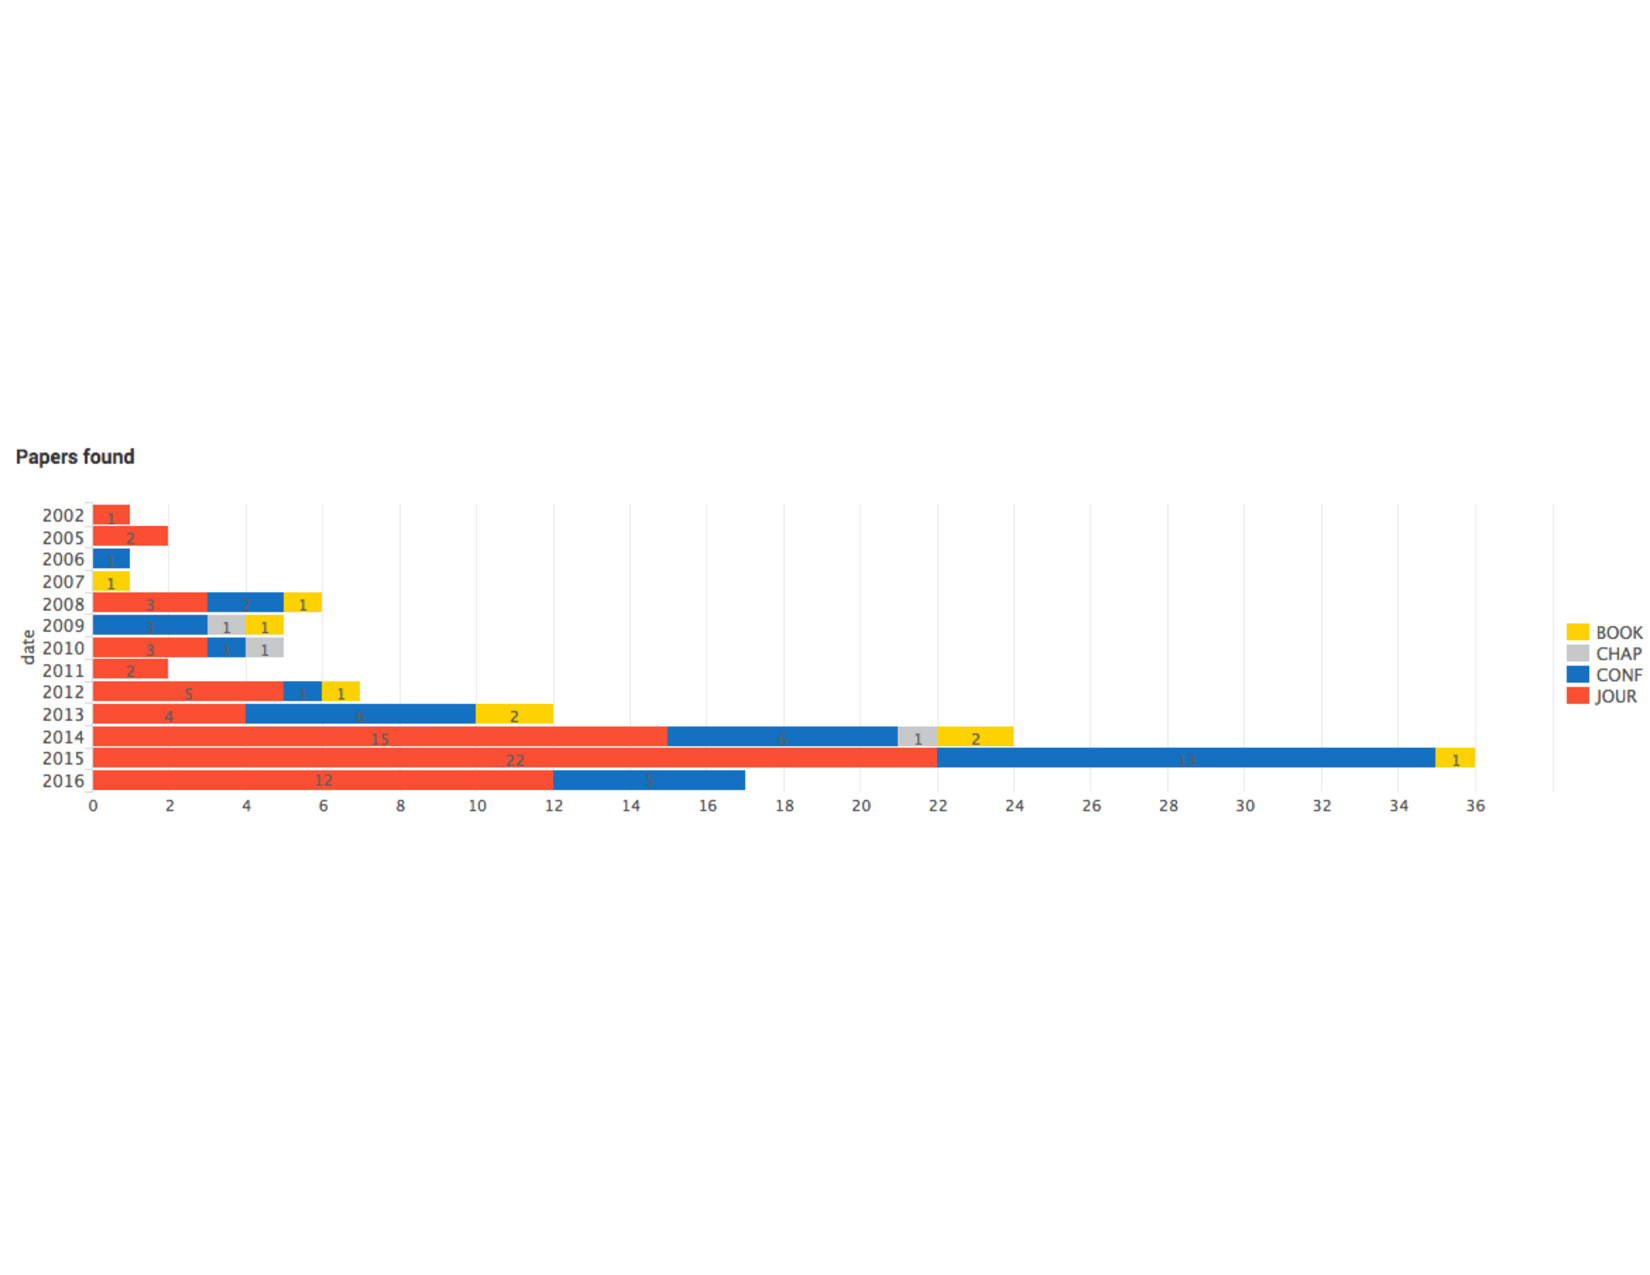
\includegraphics[width=\textwidth]{rq1}
	\caption{Distribución de los documentos por tiempo y por tipo. Captura tomada de la aplicación library.}
	\label{rq1}
\end{figure}

En la gráfica \ref{rq1}, se mostró una tendencia en los últimos tres años, el protagonismo de los documentos encontrados en las memorias de las conferencias y talleres es notorio seguido de las revistas indexadas. Para los investigadores es interesante saber que hay una demanda en los temas que abarcan la ingeniería de software, el reuso y la variabilidad. De la misma manera, todo lo que se considera en \textit{Big Data \& IoT } esta tomando fuerza. Por otra parte, no se descarta la idea de la simplicidad y la rapidez de publicación, como criterio de elección para el lugar, como se muestra en la tabla \ref{rq2},  puede ser mucho mas fácil para un investigador realizar un aporte en las memoria de las conferencias a desarrollar un capitulo en un libro. Por esta razón nos preguntamos.

\paragraph{RQ2: ¿Qué tipo de documentos hablan del papel de la minería de datos en la ingeniería de líneas de producto?}
 
Los tipos de documentos encontrados varían en el tiempo pero presentan una tendencia a ser artículos de revistas indexadas y memorias en las conferencias, se quiso resaltar las palabras claves mas polulares en la gráfica \ref{keywords}, que nos ayudarán en la construcción de nuestro \textit{Quasi-Gold}, como también los diferentes lugares de publicación presentes en la tabla \ref{rq2} 

\begin{figure}[h]
	\centering
	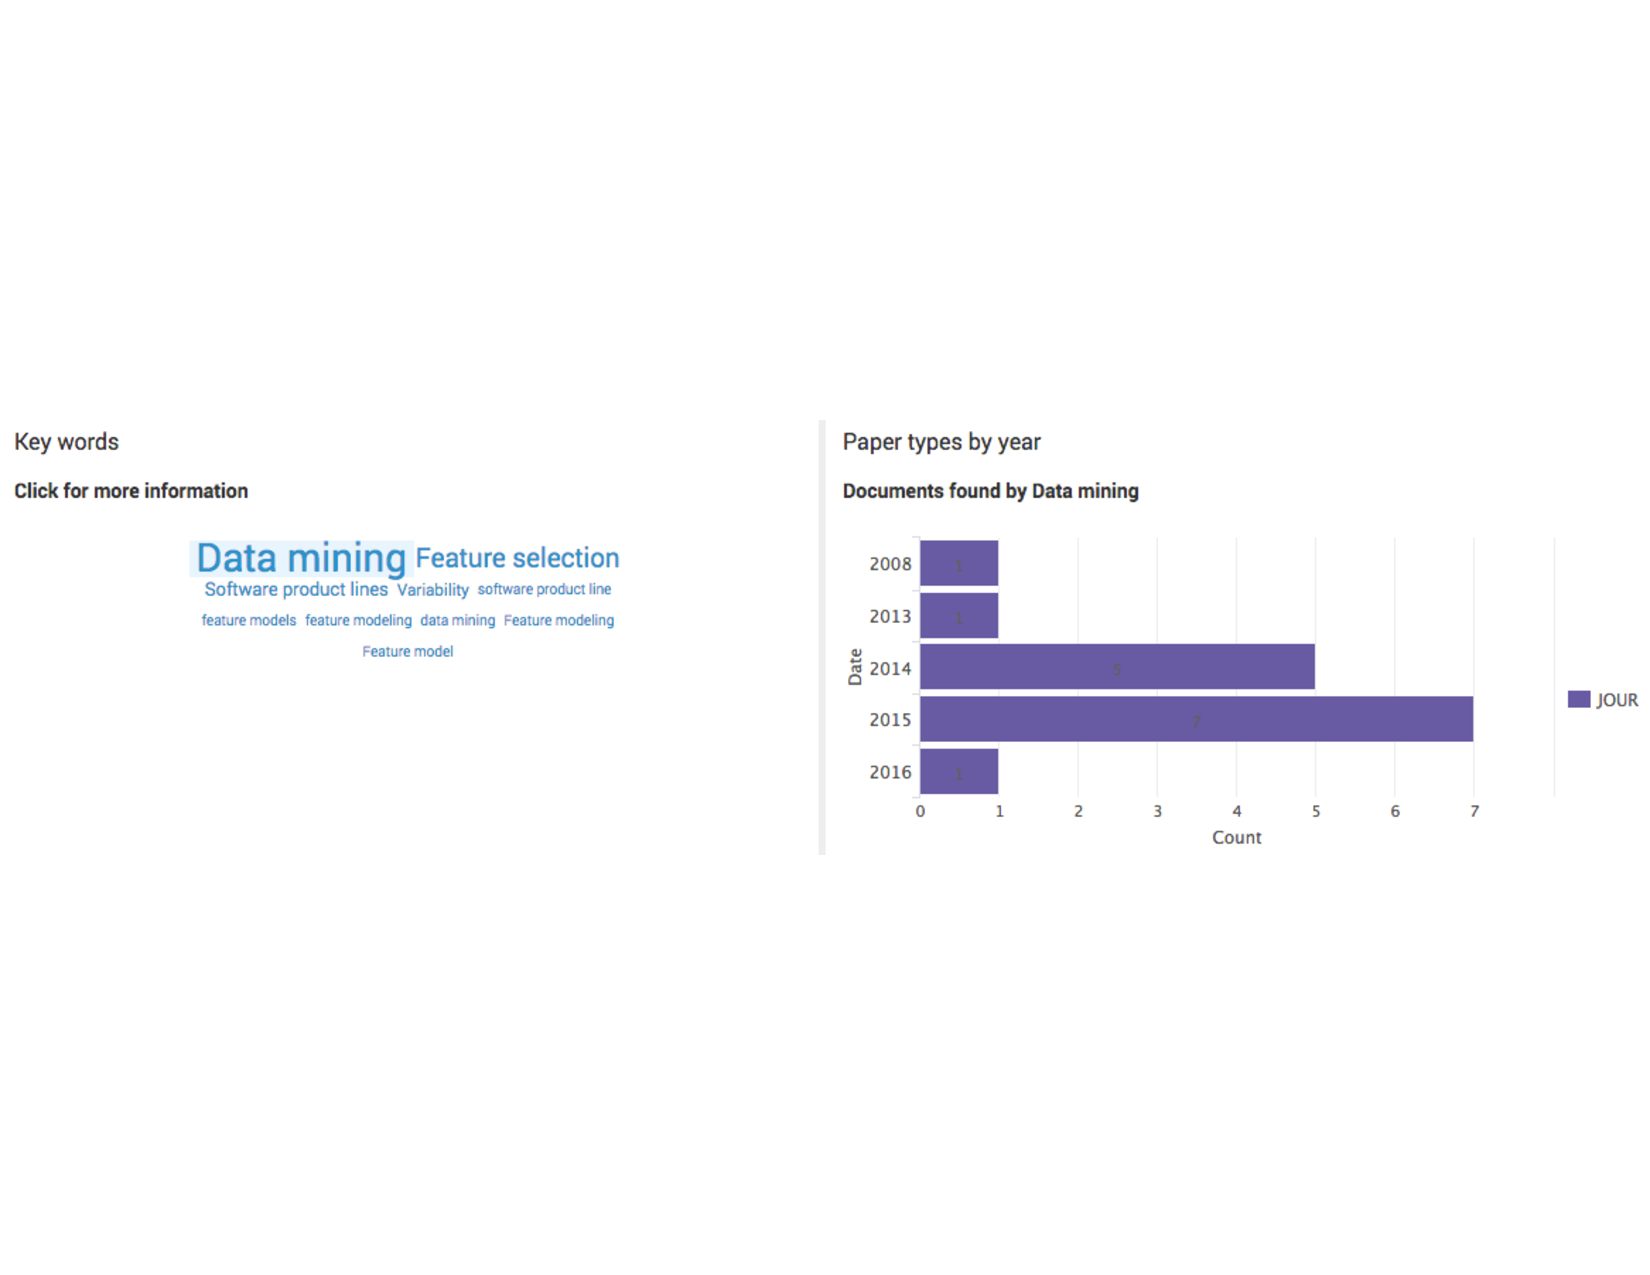
\includegraphics[width=\textwidth]{keywords}
	\caption{Captura de las sección de palabras claves en la aplicación library.}
	\label{keywords}
\end{figure}


\begin{longtable}{|p{11cm}|c|}
	\caption{Cantidad de documentos encontrados en los diferentes Lugares de publicación a lo largo del tiempo}\label{rq2}\\
	\hline
	\textbf{Lugar} & \textbf{Cantidad}  \\
	\hline
	\endfirsthead
	\multicolumn{2}{c}%
	{\tablename\ \thetable\ -- \textit{Continued from previous page}} \\
	\hline
	\textbf{Lugar} & \textbf{Cantidad}  \\
	\hline
	\endhead
	\hline \multicolumn{2}{r}{\textit{Continued on next page}} \\
	\endfoot
	\hline
	\endlastfoot
	Expert Systems with Applications                                                                                                                                                        & 8        \\ \hline
	Journal of Mechanical Design                                                                                                                                                            & 4        \\ \hline
	Proceedings of the 19th International Conference on Software Product Line - SPLC '15                                                                                                    & 4        \\ \hline
	Proceedings of the Tenth International Workshop on Variability Modelling of Software-intensive Systems - VaMoS '16                                                                      & 4        \\ \hline
	Information Sciences                                                                                                                                                                    & 3        \\ \hline
	Information and Software Technology                                                                                                                                                     & 3        \\ \hline
	Proceedings of the Ninth International Workshop on Variability Modelling of Software-intensive Systems - VaMoS '15                                                                      & 3        \\ \hline
	2008 12th International Software Product Line Conference                                                                                                                                & 2        \\ \hline
	2013 4th International Workshop on Product LinE Approaches in Software Engineering (PLEASE)                                                                                             & 2        \\ \hline
	ACM Computing Surveys                                                                                                                                                                   & 2        \\ \hline
	Applied Soft Computing                                                                                                                                                                  & 2        \\ \hline
	Empirical Software Engineering                                                                                                                                                          & 2        \\ \hline
	IEEE Transactions on Software Engineering                                                                                                                                               & 2        \\ \hline
	Knowledge-Based Systems                                                                                                                                                                 & 2        \\ \hline
	Neurocomputing                                                                                                                                                                          & 2        \\ \hline
	Proceedings of the 18th International Software Product Line Conference on Companion Volume for Workshops Demonstrations and Tools - SPLC '14                                            & 2        \\ \hline
	Proceedings of the Eighth International Workshop on Variability Modelling of Software-Intensive Systems - VaMoS '14                                                                     & 2        \\ \hline
	Requirements Engineering                                                                                                                                                                & 2        \\ \hline
	2009 17th IEEE International Requirements Engineering Conference                                                                                                                        & 1        \\ \hline
	2009 International Conference on Information and Multimedia Technology                                                                                                                  & 1        \\ \hline
	2010 Seventh International Conference on Fuzzy Systems and Knowledge Discovery                                                                                                          & 1        \\ \hline
	2011 37th EUROMICRO Conference on Software Engineering and Advanced Applications                                                                                                        & 1        \\ \hline
	2013 IEEE 14th International Conference on Information Reuse \& Integration (IRI)                                                                                                       & 1        \\ \hline
	2014 10th International Conference on Natural Computation (ICNC)                                                                                                                        & 1        \\ \hline
	2014 40th EUROMICRO Conference on Software Engineering and Advanced Applications                                                                                                        & 1        \\ \hline
	2014 Second IEEE Working Conference on Software Visualization                                                                                                                           & 1        \\ \hline
	2015 12th International Conference on Fuzzy Systems and Knowledge Discovery (FSKD)                                                                                                      & 1        \\ \hline
	2015 IEEE 22nd International Conference on Software Analysis Evolution and Reengineering (SANER)                                                                                        & 1        \\ \hline
	2015 IEEE International Conference on Industrial Engineering and Engineering Management (IEEM)                                                                                          & 1        \\ \hline
	2015 IEEE Second International Workshop on Artificial Intelligence for Requirements Engineering (AIRE)                                                                                  & 1        \\ \hline
	Advanced Engineering Informatics                                                                                                                                                        & 1        \\ \hline
	Advances in Product Family and Product Platform Design                                                                                                                                  & 1        \\ \hline
	Applied Computing and Informatics                                                                                                                                                       & 1        \\ \hline
	Applied Energy                                                                                                                                                                          & 1        \\ \hline
	CEUR Workshop Proceedings                                                                                                                                                               & 1        \\ \hline
	Collaboration and Technology                                                                                                                                                            & 1        \\ \hline
	Computer Standards \& Interfaces                                                                                                                                                        & 1        \\ \hline
	Computer-Aided Design                                                                                                                                                                   & 1        \\ \hline
	Computers \& Chemical Engineering                                                                                                                                                       & 1        \\ \hline
	Computers and Electronics in Agriculture                                                                                                                                                & 1        \\ \hline
	Construction and Building Materials                                                                                                                                                     & 1        \\ \hline
	Control Engineering Practice                                                                                                                                                            & 1        \\ \hline
	DYNA                                                                                                                                                                                    & 1        \\ \hline
	Elements                                                                                                                                                                                & 1        \\ \hline
	Engineering Applications of Artificial Intelligence                                                                                                                                     & 1        \\ \hline
	Evolving Software Systems                                                                                                                                                               & 1        \\ \hline
	Information Systems                                                                                                                                                                     & 1        \\ \hline
	International Journal of Electrical Power \& Energy Systems                                                                                                                             & 1        \\ \hline
	International Journal of Forecasting                                                                                                                                                    & 1        \\ \hline
	Journal of Computing and Information Science in Engineering                                                                                                                             & 1        \\ \hline
	Journal of Retailing and Consumer Services                                                                                                                                              & 1        \\ \hline
	Journal of Software: Evolution and Process                                                                                                                                              & 1        \\ \hline
	Journal of Systems and Software                                                                                                                                                         & 1        \\ \hline
	Journal of Testing and Evaluation                                                                                                                                                       & 1        \\ \hline
	Journal of the Brazilian Computer Society                                                                                                                                               & 1        \\ \hline
	Journal of the Royal Statistical Society: Series B (Statistical Methodology)                                                                                                            & 1        \\ \hline
	Lecture Notes in Computer Science (including subseries Lecture Notes in Artificial Intelligence and Lecture Notes in Bioinformatics)                                                    & 1        \\ \hline
	Nature                                                                                                                                                                                  & 1        \\ \hline
	Pattern Recognition                                                                                                                                                                     & 1        \\ \hline
	Performance Evaluation                                                                                                                                                                  & 1        \\ \hline
	Proceedings - 40th Euromicro Conference Series on Software Engineering and Advanced Applications SEAA 2014                                                                              & 1        \\ \hline
	Proceedings of the 16th International Conference on Computer Systems and Technologies - CompSysTech '15                                                                                 & 1        \\ \hline
	Proceedings of the 18th ACM SIGKDD international conference on Knowledge discovery and data mining - KDD '12                                                                            & 1        \\ \hline
	Proceedings of the 18th International Software Product Line Conference on - SPLC '14                                                                                                    & 1        \\ \hline
	Proceedings of the 19th International Conference on Evaluation and Assessment in Software Engineering - EASE '15                                                                        & 1        \\ \hline
	Proceedings of the 19th International Conference on Software Product Line                                                                                                               & 1        \\ \hline
	Proceedings of the 2009 ACM symposium on Applied Computing - SAC '09                                                                                                                    & 1        \\ \hline
	Proceedings of the 2012 International Symposium on Computers in Education (SIIE)                                                                                                        & 1        \\ \hline
	Proceedings of the 2015 International Conference on Software and System Process - ICSSP 2015                                                                                            & 1        \\ \hline
	Proceedings of the 23rd international conference on Machine learning - ICML '06                                                                                                         & 1        \\ \hline
	Proceedings of the 31st Annual ACM Symposium on Applied Computing - SAC '16                                                                                                             & 1        \\ \hline
	Proceedings of the IEEE                                                                                                                                                                 & 1        \\ \hline
	Proceedings of the Ninth International Workshop on Variability Modelling of Software-intensive Systems                                                                                  & 1        \\ \hline
	Proceedings of the Seventh International Workshop on Variability Modelling of Software-intensive Systems - VaMoS '13                                                                    & 1        \\ \hline
	Proceedings of the Tenth International Workshop on Variability Modelling of Software-intensive Systems                                                                                  & 1        \\ \hline
	Proceedings of the \{ER\} 2009 Workshops (\{CoMoL\} \{ETheCoM\} \{FP-UML\} \{MOST-ONISW\} \{QoIS\} \{RIGiM\} \{SeCoGIS)\} on Advances in Conceptual Modeling - Challenging Perspectives & 1        \\ \hline
	Remote Sensing of Environment                                                                                                                                                           & 1        \\ \hline
	Scientific Reports                                                                                                                                                                      & 1        \\ \hline
	Software Product Lines in Action: The Best Industrial Practice in Product Line Engineering                                                                                              & 1        \\ \hline
	Statewide Agricultural Land Use Baseline 2015                                                                                                                                           & 1        \\ \hline
	The 7th International Conference on Information Technology                                                                                                                              & 1        \\ \hline \bottomrule
\end{longtable}


Continuamos con el análisis de los autores mas representativos de nuestros resultados y, nos preguntábamos.
\paragraph{RQ3: ¿Qué distribución geográfica o cuales autores son los mas representativos en nuestro estudio?}
Con el propósito de conocer las personas que pueden estar interesadas en nuestro proyecto de investigación, descubrimos la siguiente distribución geográfica para los autores mas populares de nuestro MSL como se muestra en la figura \ref{rq3}. 
\begin{figure}[h]
	\centering
	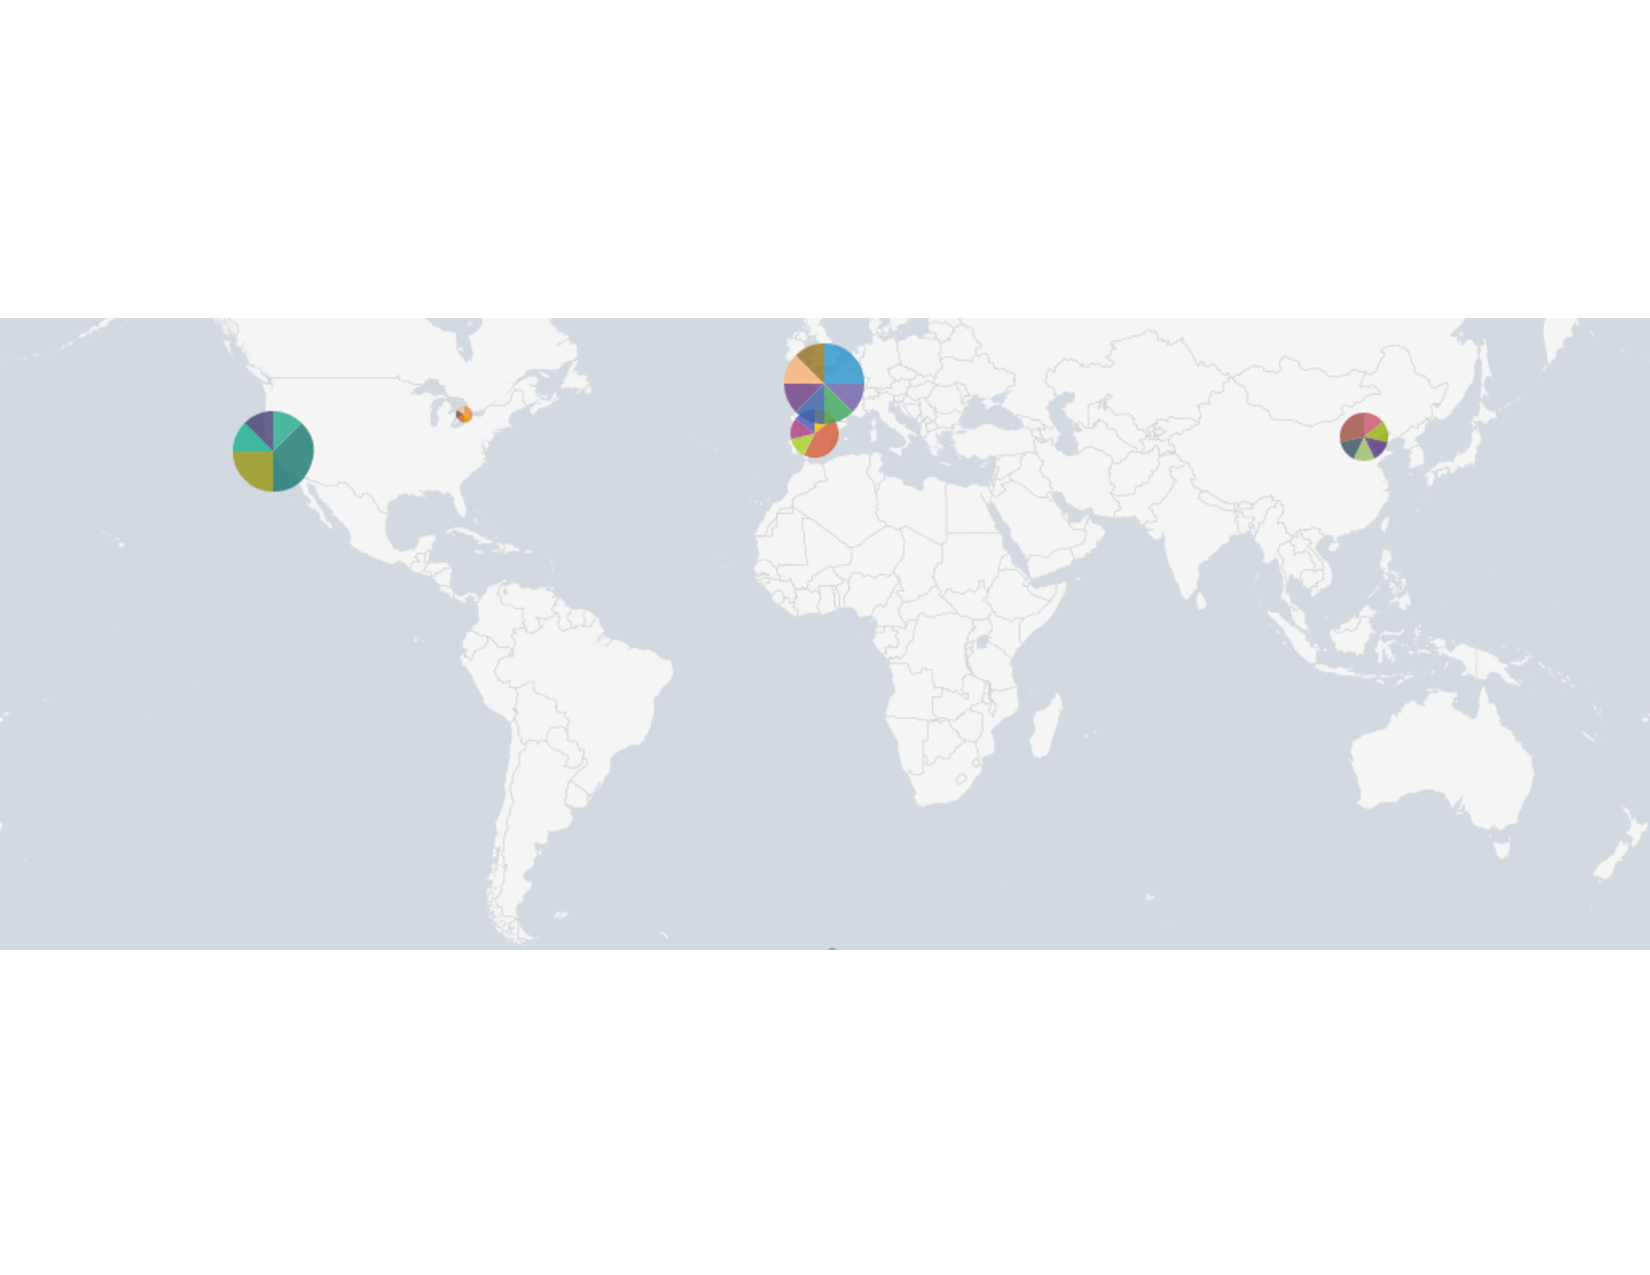
\includegraphics[width=\textwidth]{rq3}
	\caption{Captura de la sección donde se muestra la  ubicación geográfica de autores según su universidad, tomada en la aplicación library.}
	\label{rq3}
\end{figure}

 Mathieu Acher de la Université de Rennes 1, Rennes, Francia con cinco documentos en los cuales destaca un capítulo del libro \textit{Lecture Notes in Computer Science}\cite{Acher2010}. Desde Martin Becker de Fraunhofer-Platz 1, Kaiserslautern, Alemania que destaca con Bo Zang de la University of Kaiserslautern, Alemania por \textit{RECoVar}\cite{Zhang2013}  y sus diversas contribuciones en los talleres sobre variabilidad en la ingeniería del software. También tenemos a Guillaume Bécan de Université de Rennes 1 en Rennes, Francia con un articulo muy interesante \textit{On breaking the curse of dimensionality in reverse engineering feature models}\cite{Davril2015}, Rafael Capilla de Rey Juan Carlos University en Madrid, España propone  administrar la variabilidad en la ingeniería de software desde su libro \textit{Systems and Software Variability Management}\cite{Capilla2013} , Krzysztof Czarnecki de University of Waterloo, en la provincia de Ontario en Canada trabaja en las conferencias y talleres sobre minería de datos, Trevor Hastie de Stanford University en California, U.S.A., es un contribuyente excepcional al aprendizaje de maquina, con diferentes libros de una calidad sin paragón como \textit{The elements of  statistical learning}\cite{Hastie2009} se convirtió en el texto guía para muchos estudios y cursos, Raúl Mazo y Camille Salience  de Université Paris 1 Panthéon-Sorbonne, Paris, Francia con artículos como \textit{Reusable knowledge in security requirements engineering: a systematic mapping study}\cite{Souag2015} y memorias en conferencias como VariaMos\cite{Mazo2015}, protagonizan las regiones y las personas con las cuales podemos construir alianzas estratégicas y futuros trabajos.

Con el fin de establecer un grado de madurez para el tema de investigación como lo propone Roel Wieringa, \textit{et al.} \cite{Wieringa2006}.  Proponemos la siguiente pregunta de investigación.
\paragraph{RQ4: ¿Qué categoría o escalafón de investigación tienen asignado los documentos encontrados en nuestro estudio?}
Basados en la cantidad de citas como se muestra en la figura \ref{rq4}, pudimos determinar algunos estudios importantes. 
\begin{figure}[h]
	\centering
	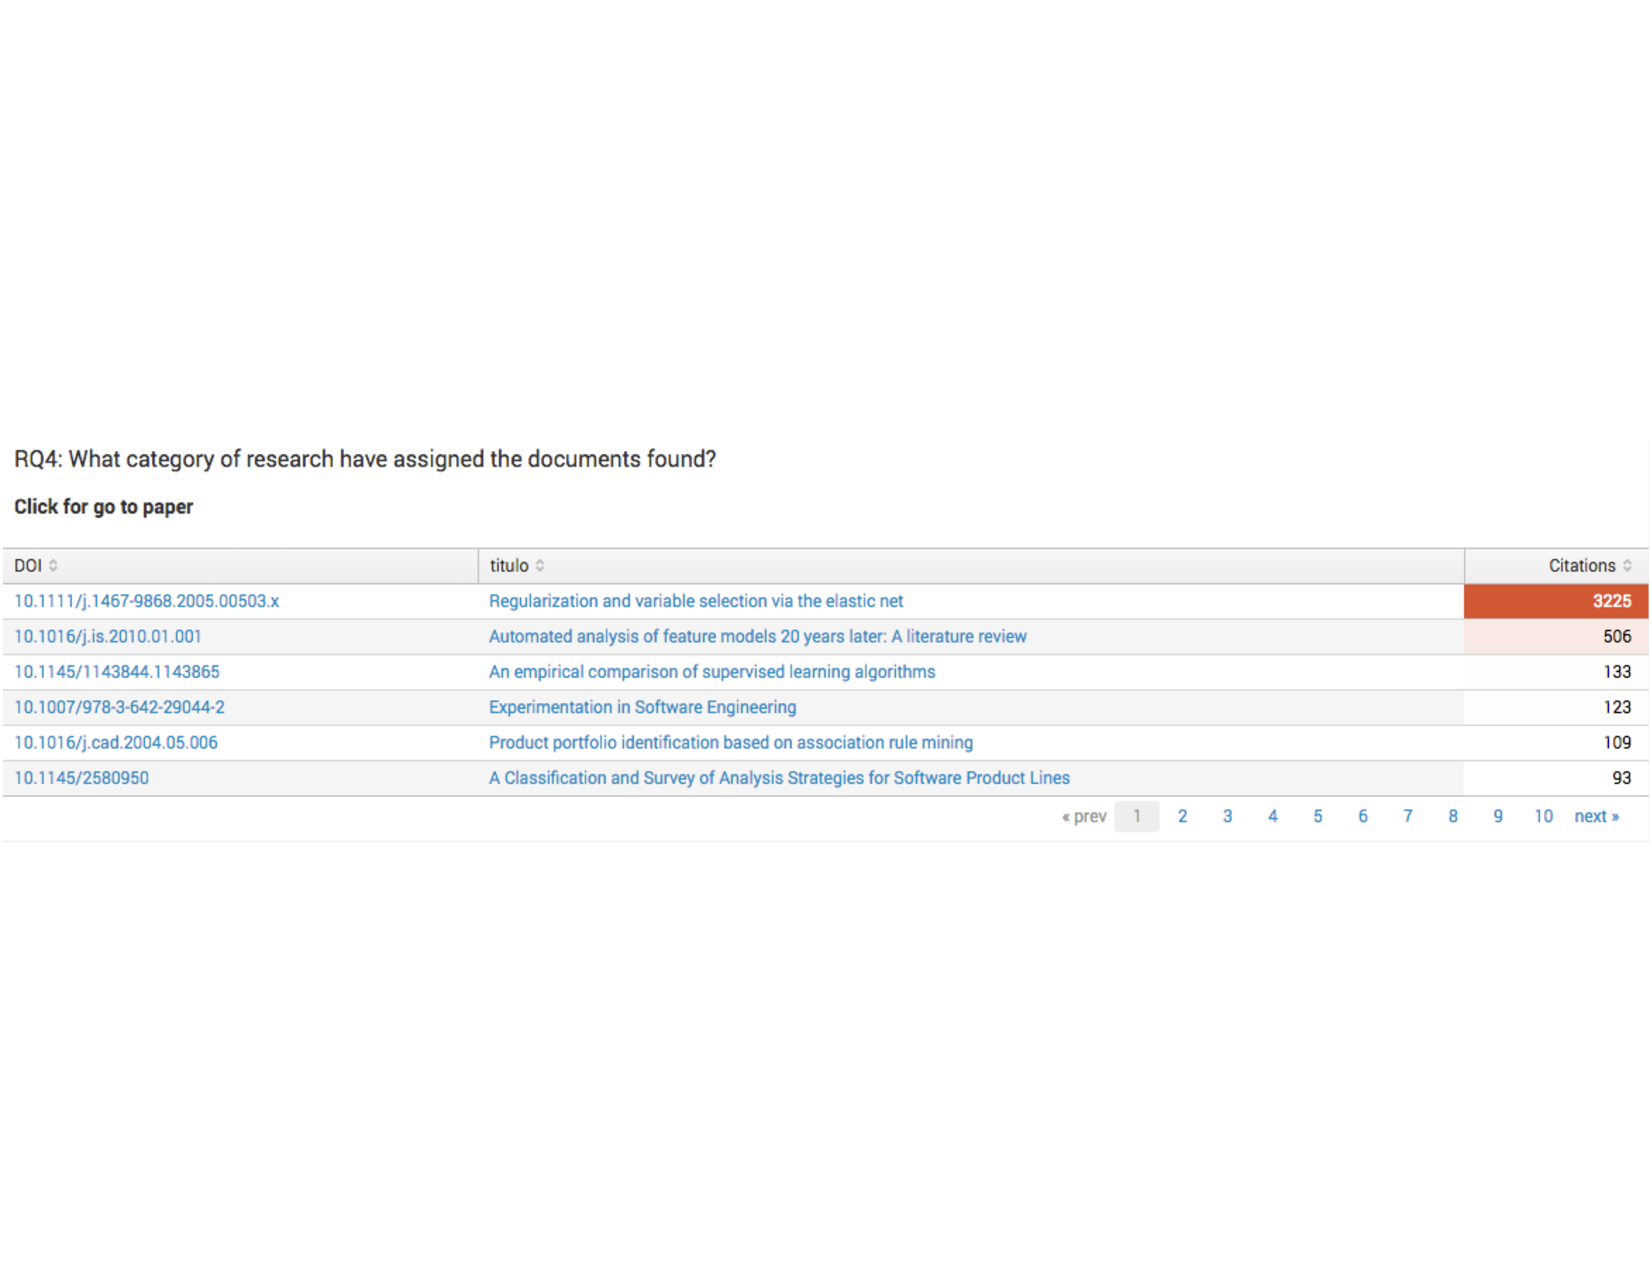
\includegraphics[width=\textwidth]{rq4}
	\caption{Captura de la sección donde se muestra en orden descendente los documentos según su cantidad de citas, tomada en la aplicación library.}
	\label{rq4}
\end{figure}

Descubrimos que en el campo de la MD y el \textit{machine learning}, existe una comunidad vibrante de investigadores, es decir que hay personas muy apasionadas por generar conocimiento y, un ejemplo de la madurez de estos trabajos es \textit{Regularization and variable selection via the elastic net}\cite{Zou2005a}, donde se parte desde los avances de Leo Brieman y Trevor Hastie. En esta publicación se recuerda que desde la suma de cuadrados se pueden seleccionar los valores que mas aportan en la varianza de de las observaciones, se pasa por los métodos de selección de las variables como lo hace  \textit{Lasso} o \textit{LARS algorithm} para proponer  un acercamiento a los problemas que ocasiona la maldición de la dimesionalidad: Donde se tienen mas factores que muestras. Y como darle solución mediante la  penalización de los coeficientes de los factores de que no aporten tanto a la suma de cuadrados. 
Siguiendo con el tema de la MD y teniendo en cuenta que  todo trabajo de investigación necesita justificar las herramientas que se usan o se proponen, es común que un ingeniero busque la mejor herramienta, por esta razón consideramos a Rich Caruana y a Alexandru Niculescu-Mizil en \textit{An empirical comparison of supervised learning algorithms}\cite{Caruana2006}  donde se descubren las justificaciones para usar \textit{ramdon forest} en la solución de los problemas con aprendizaje supervisado como el que se desarrollo en este proyecto de investigación con los RIPS.
Por otra parte,  en el campo del desarrollo de software tenemos el inconveniente de que casi todos los enfoques novedosos son publicados en eventos industriales como \textit{Summit's}, por ejemplo en el caso de Apple esta \textit{The Apple Worldwide Developers Conference (WWDC)} o el \textit{Google I/O} en Google y en el caso de los videojuegos tenemos  el \textit{E3 - Electronic Entertainment Expo} para la presentación de estos avances. Sin embargo, las editoriales nunca están demasiado lejos cuando se trata de publicar documentos que cuenten como se generan productos personalizados de forma masiva, problema por el cual los modelos de características son la opción mas popular en los últimos años y por esto no fue raro encontrar una gran comunidad siguiendo los trabajos de David Benavides, \textit{et al.}, como ejemplo tenemos \textit{Automated analysis of feature models 20 years later: A literature review}\cite{Benavides2010}.
En este trabajo de investigación se encontró que la ILP se usa en numerosos contextos de negocio igual que la MD, por esta razón identificamos estas coyunturas.
\paragraph{RQ5: ¿Qué algoritmos o técnicas son usadas en el ciclo de vida de la ingeniería de líneas de producto para crear modelos de características?} 
Considerando el \textit{framework} propuesto por Jianxin (Roger) Jiao en \textit{Advances in Product Family and Product Platform Design}\cite{Simpson} sabemos que la ILP es un proceso que se le conoce por un ciclo de vida y este puede aplicarse en cualquier contexto. La literatura muestra la transformación del ciclo de vida de ILP a travez del tiempo, donde inicialmente se planteo en el mundo del software(\textit{Software Product Lines in Action}\cite{VanDerLinden2007}), pero como toda organización puede modelar sus procesos de negocio como un software, este tomo protagonismo y ahora se usa en la mayoría de los industrias y con el  la ILP, esto permitió que atravez de la ILP surgieran los modelos de características como respuesta al modelado de la variabilidad de los productos en las industrias, esta pregunta se detiene en este punto, acá, proponemos hacer un alto y contemplar como las técnicas de minería de datos se usan para crear modelos de características.
\begin{itemize}
	\item{ \textbf{Data Mining-Driven Product Design:}}
	Iniciamos con \textit{Advances in Product Family and Product Platform Design}\cite{Simpson} donde Timothy W Simpson y Jianxin Roger Jiao nos recordaron el campo emergente \textit{data mining-driven product design} el cual tiene como objetivo incorporar a los grandes volúmenes de datos en el proceso de diseño de los productos, por ejemplo, emplear \textit{clustering} para el agrupamiento de las funciones de los productos con el fin de crear familias de productos, usar \textit{Naive Bayes Classification} para la creación de productos, escogiendo entre muchas características las combinaciones de ellas que se consideran  novedosas, utilizar \textit{data mining Fuzzy c clustering techniques} como una estrategia de identificación de plataformas en el diseño de una familia de productos o proponer un \textit{Data Mining framework} para extraer el conocimiento con el fin de crear plataformas de productos, entre otros. 
	\item{ \textbf{Feature-Oriented Modeling Aproach:}} 
	Yang Guanzhong y Zhang Yaru en \textit{A feature oriented modeling approach for embedded product line engineering}\cite{Yang2015a} propone describir las características de los productos de manera detallada mediante un proceso de modelado de características que inicialmente se divide en dos partes, análisis del dominio y análisis de requerimientos, con esto se pasa a un modelo conceptual de dominio que permitirá el análisis de las características. Este análisis se extraen las relaciones entre características y su variabilidad e inmutabilidad, luego, se construye el modelo de características y se valida. En este documento se tienen en cuenta las propuestas tradicionales como \textit{Feature Oriented Domain Analysis (FODA)}, \textit{Feature-Oriented Domain Model(FODM)} \& \textit{Feature  Oriented Reuse Method (FORM)} para proponer, que en las lineas de producto embebidas se pueden extender de las características de los productos un conjunto de conceptos, características y atributos. Con todo esto en mente, la vista de un modelo de características quedaría dividida en tres partes, modelo de características funcionales, modelos de características no-funcionales y modelo de características del sistema. Las relaciones entre estos modelos especificará la consistencia o la flexibilidad en la variabilidad de la línea de productos.
	En \textit{Code Smells Revisited: A Variability Perspective}\cite{Fenske2015} Wolfram Fenske y Sandro Schulze describen que la variabilidad que tiene de un modelo de características y la detección de errores en el software, se puede considerar con FODA, el enfoque de anotaciones y el de los mecanismos basados en composiciones.
	\item{ \textbf{Evolution of Software Product Lines:}}
	Al analizar la evolución de la línea de productos podemos obtener una colección de modelos de caracteristicas utiles para la creación de nuevos productos, en \textit{Evolution of Software Product Lines}\cite{PeterJ.Olver2013}  Goetz Botterweck y Andreas Pleuss proponen realizar una ingeniería inversa para la creación de modelos de características iniciando por ejemplo de características sin estructura, arquitecturas o incluso descripciones informales de los productos.  El proceso que se describe en el documento anterior es complejo pero los autores lo resumen como un proceso de migración, que se compone de varios procesos mas pequeños, como el análisis de la línea de producto, la planeación de su futuro y finalmente la implementación de su evolución. Luego, como todo proceso es necesario chequear la consistencia de la línea de productos, con esto Alcemir Rodrigues Santos, \textit{et al.} presentan un resumen sistemático sobre las estrategias para chequear la consistencia en las LPS\cite{Santos2015} considerando también su evolución.
	El kernel de Linux a sido estudiado ampliamente en el contexto de la ILPS, por ejemplo Rothberg Valentin \textit{et al} en \textit{Feature Models in Linux}\cite{Rothberg2016} muestra como el funcionamiento de los componentes está supeditado a los casos de uso.  El modelo de características perteneciente al kernel de Linux es una colección de mas de $15200$ caracteristicas que crece cada día, y en su evolución fueron creados los modelos de características que representan su línea de productos. En este documento se presenta un marco de trabajo (\textit{FMDiff}) que realiza operaciones de división y comparación para clasificar y analizar los cambios en el kernel, luego se emplea \textit{Kconfig extractor dumpconf from the undertaker suite} para generar el modelo de características según la arquitectura en \textit{Rigi Standard Format (RSF)}. Finalmente cuando se cuenta con el modelo de características en el formato RSF se pueden seguir haciendo las comparaciones y darle continuidad al proceso de evolución.
	\item{ \textbf{Ingeniería inversa de la variabilidad y las configuraciones:}}
	Esta técnica obedece al \textit{framework: RECoVar}\cite{Zhang2013} propuesto por Bo Zhang y Martin Becker  que tiene como objetivo general el incremento de la productividad en la línea de productos de software y librarse de la erosión en los artefactos durante la evolución de la LPS, este framework incluye dos enfoques el primero es la extración del modelos de varibilidad basado ene l código, mientras que el segundo identifica las correlaciones complejas en las caracteristicas presentes en la configuracion de la LPS. para el proceso de minería de datos usan \textit{the Orange tool} y en los trabajos futuros no descartan la idea de usar los modelos de caracteristicas probabilisticos (\textit{Probabilistic Feature Model (PFM)}) para la extración de las configuraciones que involucren la correlación entre características.
	\item{ \textbf{The Feature Mining process:}}
	La ingeniería inversa para la adquisición de un modelo de características realizada de manera manual puede consumir mucho tiempo, ser propensa a errores y requerir mucho esfuerzo, por esta razón Ra'Fat AL-Msie'Deen, \textit{et al.}\cite{Al2013} proponen que si se necesita explotar las variantes existentes en un software para la construcción de una línea de productos de software, se debe realizar un \textit{Formal Concept Analysis (FCA)} y luego extraer su variabilidad mediante la combinación de la similaridad lexica y estructural de sus \textit{object-oriented building elements(OBE's)}. Para realizar esto Ra'Fat AL-Msie'Deen, \textit{et al.}\cite{Al2013} usaron una \textit{Dependency Structure Matrix (DSM)}, para establecer las dependencias entre las clases(\textit{OBE's}), para analizar las dependencias y extraer los \textit{OBE's} usaron \textit{Eclipse Java Development Tools (JDT)}, presentaron los \textit{OBE's} con la librería \textit{JDOM} en el formato \textit{XML}, para aplicar \textit{FCA} usaron \textit{Eclipse eRCA platform}  y para la similaridad léxica crearon su propia técnica de \textit{Latent semantic analysis (LSA)} basada aparentemente en un algoritmo de \textit{Cluster K-means}, luego representa su modelo de características en un \textit{Eclipse plug-in for Feature-Oriented Software Development.} llamado \textit{FeatureIDE}  o en \textit{ArgoUML-SPL}.
	Tambien podemos considerar que en la construcción automática de los modelos de características en donde se tiene en cuenta la maldición de la dimensionalidad o la alta dimensionalidad\cite{Maldonado2014}, se pueden aplicar algoritmos de reducción de dimensión con la motivación de sintetizar la información las variables y obtener la información relevante desde las matrices de configuración como se muestra en \textit{On breaking the curse of dimensionality in reverse engineering feature models}\cite{Davril2015}  por Jean Marc Davril, \textit{et al.}
	En \textit{Feature model augmentation with sentiment analysis for product line planning}\cite{Zhou2015b} debido a la compilación de grandes volúmenes de información sobre las preferencias de los clientes, Feng Zhou y Jianxin (Roger) Jiao realizaron un análisis de sentimientos sobre las preferencias de los clientes al comprar en una tienda en línea, con el objetivo de incorporar los gustos de los clientes en el proceso de construcción de un modelo de características.Como se ve tambien en \textit{Mining customer knowledge for product line and brand extension in retailing}\cite{Liao2008}, este método que se propone en el documento anterior también buscaba mejorar la eficiencia y la calidad en la planeación de la línea de productos, en lugar de hacerlo por el camino tradicional que se indica en la ingeniería de requisitos.
	\item{ \textbf{The domain analysis process:}}
	Auque esta es una etapa dentro del ciclo de vida del desarrollo de software, esencial en el desarrollo de la línea de productos, Negar Hariri, \textit{et al.}\cite{Hariri2013} propone usar el descubrimiento de información en las bases de datos para la creación de modelos de dominio que bien se pueden procesar para crear modelos de características. En este trabajo se propone usar algoritmos de agrupamiento difusos, que combinados con técnicas de extracción de reglas de asociación como \textit{kNN} pueden recomendar características que deberían estar presentes en la construcción de futuros productos.
	\item{ \textbf{Composition Operators:}}
	Como el proceso de análisis del dominio, presentado anteriormente, estas operaciones sobre los modelos de características (MC) no fueron en sí usadas desde su concepción para la creación de dichos modelos; fue con la aparición del problema de la alta dimensional en los datos, en el desarrollo de la ingeniería de líneas de producto que se construían MC grandes y monolíticos, este proceso fue muy incomodo, propenso a errores y muy costoso para las diferentes partes interesadas en el desarrollo de la línea de productos. Con el fín de manejar la alta dimensionalidad los MC fueron separados y \textit{composed} por varias operaciones con el objetivo de no perder la integridad cuando sean separados o unidos nuevamente. Esta filosofía de dividir y vencer dio a conocer dos operaciones basicas: \textit{insert} \& \textit{merge} que se comparan al detalle en \textit{Comparing Approaches to Implement Feature Model Composition}\cite{Acher2010} en donde Mathieu Acher propone considerar otras dos operaciones \textit{diff} \& \textit{refactoring} nosotros pensamos que la derivación de los modelos de caracteristicas mediante sus operaciones pueden generar nuevos elementos y con ellos, nuevos MC.
	\item{ \textbf{Variability management:}}
	Es una actividad que dentro de la ingeniería de líneas de productos maneja el conocimiento racional para la toma de decisiones entre las diferentes partes interesadas en en un proyecto de ILP, con esto nos referimos a que la \textit{Variability management} es una rama de la ciencia que se basa en los argumentos, las razones y las justificaciones detrás de cada decisión que toman los interesados. Anil Kumar Thurimella y  Bernd  Bruegge proponen la metodología \textit{issue-based variability management methodology (IVMM)}\cite{Thurimella2012} que combina preguntas, opciones y criterios.
	\item{\textbf{The multi-level feature model:}}
	En \textit{Cross domain web information extraction with multi-level feature model}\cite{Chen2014a}, Qian Chen  propone que para manejar las características efectivamente, se debe hacer énfasis en las relaciones que aparezcan en la configuración del dominio, con estas relaciones  se propone crear un modelo que permita la extracción de características considerando los cambios en el dominio. Esto incrementa la adaptabilidad y el reuso de las características en el modelo. Este es un modelo teórico de una estructura jerarquica que puede derivar modelos de características.
	\item {\textbf{Automated feature model configuration:}}
	Mohsen Asadi, \textit{et al.} en \textit{Toward automated feature model configuration with optimizing non-functional requirements}\cite{Asadi2014} establece la idea de emplear tecnicas de planeación para solucionar un problema de configuración, en este documento se transforman los modelos de características, mediante una tecnica de planeación en  inteligencia artificial conocida como \textit{Hierarchical Task Network (HTN) Planning} para que automáticamente seleccione las características mas relevantes para los interesados. En este documento se establece que el proceso de configuración del árbol de características estará dado por los requisitos funcionales y no-funcionales que se persiven en las necesidades de los interesados.
	\item {\textbf{Extracción de características desde el lenguaje natural:}}
	Noor Hasrina Bakar, \textit{et al.} propone una completa colección de las técnicas usadas para extraer las características en el lenguaje natural de los requisitos en la ingeniería de líneas de producto de software\cite{Bakar2015a}, este estado del arte es relevante debido a que en él, se considera que las técnicas usadas para el descubrimiento y agrupamiento de las características ya sea desde la minería de datos, las técnicas automáticas y manuales, aún no están disponibles totalmente para la comunidad. Por otra parte, muchas de las técnicas carecen de una validación o de un caso practico. En consecuencia, muchos interesados en el tema aún siguen extrayendo las características mediante la ingeniería de requisitos.
	\item {\textbf{Antologias:}}
	En el documento de Lamia Abo Zaid, \textit{et al.} \textit{Applying semantic web technology to feature modeling}, se parte de que introducir y administrar la variabilidad en los productos de software por ejemplo, no es una tarea trivial, pueden existir muchas variaciones de los productos y mediante diferentes notaciones se puede representar la misma información, por esta razón representar los modelos de características para un sistema puede llegar a ser muy complicado.
	Una antología representa el conocimiento de cierto dominio mediante clases, propiedades y restricciones. Considerando lo anterior en este documento se propone usar un framework para la construcción de modelos de características usando \textit{web ontology language (OWL)}.
	\item {\textbf{Variability modeling Techniques:}}
	En \textit{A survey of variability modeling in industrial practice}\cite{Berger2013},  Thorsten Berger, \textit{et al.} presenta la respuesta a tres preguntas que se planteó en el anterior \textit{survey}, ¿Que notaciones en el modelado de la variabilidad son usadas?¿cuales son las escalas de los modelos industriales?¿Que beneficios y desafíos se perciben con el modelado de la variabilidad? Y aunque desde el 2012 el \textit{Object Management Group (OMG)} estableció un estándar para el modelamiento de la variabilidad, la comunidad ha desarrollado varios acercamientos que pretenden adaptarse a las diferentes necesidades academicas e industriales sin seguir el estándar con rigor, por consiguiente, hay una diversa variedad de notaciones en la definición de los modelos de características en la ingeniería de líneas de producto\footnote{http://www.omgwiki.org/variability/doku.php}.  
	\item {\textbf{Holistic feature modeling:}}
	Jaejoon Lee, \textit{et al.} en \textit{A holistic approach to feature modeling for product line requirements engineering}\cite{Lee2014} nos presentan la reconciliación entre la ingeniería de requisitos y la ILPS, con un enfoque que considera los problemas cotidianos y los modela mediante metas y atributos de calidad, para luego separar las características en los espacios del problema y la solución, finalmente crear el modelo de características que represente los productos de la LP. Usar modelos de metas y de características en el espacio de la solución y el problema respectivamente es un gran enfoque que proporciona múltiples puntos de vista de la LP, sistematicamente este enfoque puede establecer que las características pertenecen al espacio de la solución y los requerimientos al espacio del problema.
	\item {\textbf{Temporal Market-Driven Responses:}}
	En el proceso de extracción, carga y transformación que esta explicito en \textit{Advances in Product Family and Product Platform Design - Quantifying the Relevance of Product Feature Classification in Product Family Designe}\cite{Kwak2011} se establece que en la creación de plataformas de producto y familias de producto (Termino para referise tambien a las líneas de producto), a lo largo del tiempo deben aparecer, desaparecer y reaparecer características en los productos de acuerdo a las necesidades del mercado y siempre será interesante modelar que características se incluyen y cuales no en la próxima generación de la familia de productos.
	\item {\textbf{Configuración interactiva de modelos de características:}}
	Dadas las grandes proporciones que puede tener un modelo de características partimos de que la configuración inicial del modelo será el producto mas sencillo que cumpla con las reglas del contexto para el cual es diseñado, luego podríamos configurar productos que acarrearán mas características y por lo tanto mas complejidad. En \textit{On lazy and eager interactive reconfiguration}\cite{Janota2013}, Mikolás Janota propone que \textit{eager} provee información sobre el usuario y \textit{lazy} busque en cientos de miles de características, con esta configuración interactiva se pueden sugerir productos para públicos determinados, es necesario aclarar que con la sugerencia de estos productos no se desea limitar al consumidor, este enfoque solo quiere establecer configuraciones por defecto para agilizar sus decisiones.
	\item {\textbf{Matrices de configuración y descripción de los productos:}}
	Las descripciones de los productos son usualmente representadas en estas tablas conocidas en la literatura como \textit{configuration matrix}, este formato describe los productos con el objetivo de documentarlos y diferenciarlos. Esta representación sirve de intermediario para obtener modelos de características, en \textit{Synthesis of attributed feature models from product descriptions},  Guillaume Bécan, \textit{et al.} desarollan un algoritmo basado en los marcos de trabajo de \textit{FAMA \& FODA} para crear modelos de características llamados \textit{attributed feature models (AFMs)} desde la descripción de los productos. Como forma de validación se espera que no halla perdida de información cuando se represente la descripción del producto en forma de matriz o en la forma de modelo de características.
\end{itemize}   
Por otro lado también es interesante para el desarrollo del proyecto de investigación justificar el uso de la minería de datos en PLE, por esta razón nos hicimos el siguiente cuestionamiento.
\paragraph{RQ6: ¿Qué técnicas de minería de datos son usadas en el campo de la ingeniería de líneas de producto?}

Actualmente, diversas tecnologías almacenan los datos del proceso de ILP, estos datos son valiosos y han sido aprovechados para tomar decisiones. En este estudio exploramos los diferentes métodos, tecnicas, algoritmos y modelos que se han usado en el la construcción de líneas de producto.

\begin{itemize}
\item {\textbf{SimpleKMeans E-learning Web Miner (ElWM) example:}}
En \textit{Software Product Line Engineering for e-Learning Applications : A Case Study}\cite{Pablo2012}, Diego Pablo Sánchez, \textit{et al.} muestra que dentro del contexto de la educación, las plataformas educativas como Moodle son muy usadas por diversas instituciones y que el reuso y la variabilida de este software genera las condiciones adecuadas para la construcción de una línea de productos. En este documento se mostró como a partir de \textit{EIWM} se pudo generar una línea de productos considerando los gustos de los estudiantes por una particular actividad dentro de un curso; se generaron nuevos cursos de acuerdo al descubrimiento de los gustos por cierto material en estudiantes y profesores. Por ejemplo, \textit{E-learning Web Miner} usa \textit{EM algorithm (Expectation Maximization)} combinado con \textit{SimpleKMeans} para agrupar a los estudiantes de acuerdo a la similaridad en sus gustos.
Por otra parte tenemos a Shu-Hsien Liao, \textit{et al.} con \textit{Mining customer knowledge for product line and brand extension in retailing}\cite{Liao2008} y sus esfuerzos para entender las complicadas y sensibles demandas de los clientes sobre los catálogos de productos de Carrefour en Taiwan mediante minería de datos. Carrefour que es una empresa inmersa en el negocio del \textit{Retailing} que inicio una linea de productos con su propia marca para impactar de forma estratégica un nicho de mercado. Ellos decidieron extraer el conocimiento que se almacena en sus bases de datos. Una vez aplicaron la metodología CRIPS desde sus bases de datos relacionales hasta conseguir un \textit{datawarehouse}, continuaron con la metodología de algoritmo \textit{K-means} para implementar \text{cluster analysis}, no obstante según  \cite{Liao2008}  algoritmos como \textit{genetic algorithms, neural nets, decision trees, regression, etc.,} se pueden implementar para lograr un análisis del dominio que produzca una línea de productos para \textit{Retailing}. Sin embargo sin un análisis inteligente de los productos que consumen los clientes no es correcto afirmar que el cliente está satisfecho con los productos que compra.

\item {\textbf{Domain analysis and reuse environment (DARE):}}
El análisis del dominio es una actividad que pretende identificar, analizar, organizar y modelar las características comunes en un dominio en particular. Negar Hariri, \textit{et al.}\cite{Hariri2013} propusieron dos algoritmos para automatizar la tarea anterior, el primer algoritmo es \textit{Fast Algorithms for Mining Association Rules} y usa minería de reglas de asociación de manera no-supervisada para descubrir la afinidad de las características a lo largo de los productos y enriquecer el perfil de los mismos. El segundo algoritmo es \textit{k-nearest neighbor} el cual toma los productos con sus perfiles aumentados y ayuda a los interesados en el proyecto de ILP recomendando las características en  los productos, en el proceso de ingeniería de requisitos.

\item {\textbf{Conjunctive and disjunctive association rule mining:}}
En la construcción de modelos de características probabilisticos,  Krzysztof Czarnecki, \textit{et al.} presenta un procedimiento en \textit{Sample Spaces and Feature Models: There and Back Again.}\cite{Czarnecki2008} que aplica  \textit{conjunctive and disjunctive association rule mining} para encontrar patrones de características recurrentes, y luego generar modelos de características probabilisticos, recordemos que los modelos de cracteristicas son la representación de la LP, entonces los modelos de características probabilisticos buscan extender la funcionalidad de los modelos de características básicos con la inclusión de restricciones suaves, las restricciones suaves son configuraciones en los productos que no son obligatorias para el usuario. Las reglas de asociación son muy usadas por las herramientas de construcción de software basadas en ingeniería inversa como se explico en la pregunta anterión en \textit{the feature mining process}.
Las reglas de asociación conjuntas buscan relaciones de tipo \textit{AND} en los productos, es decir que producto implica otro, esto se conoce también como \textit{frequent itemsets}. Las reglas de asociación disyuntas buscan relaciones de tipo \textit{OR}, es decir, que productos estarán bajo una categoría y se pueden agrupar.
En \textit{Product portfolio identification based on association rule mining}, Jianxin Jiao y Yiyang Zhang\cite{Jiao2005}, propusieron que la identificación de los productos iniciales en una línea de producto o el diseño incremental del catalogo de productos, se desarrollara atraves de una identificación de los productos mediante \textit{association rule mining system (ARMS)}, donde se hizo la selección de las variables en los productos que mas se ajusten a la estrategía de mercadeo, desde los registros de las ventas pasadas y las descripciones de los productos. Estas practicas investigativas y industriales tiene como objetivo identificar la configuración optima en los productos que generan la mayor ganancia y satisfacción en los clientes, como ejemplo en \cite{Jiao2005} se presento un ejemplo de una compañia que produce motores de vibración para celulares, en donde la arquitectura ARMS diferencio las necesidades del cliente desde los requisitos funcionales y el dominio de funciones. La identificación del portafolio de producto involucró la realización de un agrupamiento de requisitos funcionales para cada necesidad del cliente. Estos agrupamientos se realizaron mediante \textit{fuzzy clustering analysis} y el mecanismo de mapeo se realizo mediante reglas de asociación.

\item {\textbf{Relational Machine Learning:}}
Maximilian Nickel, \textit{et al.} en \textit{A Review of Relational Machine Learning for Knowledge Graphs}\cite{Nickel2015} presentaron un resumen sobre como los modelos estadísticos pueden ser entrenados con grafos voluminosos, con el proposito de que cuando el modelo prediga un nuevo hecho, este se convierta en un nuevo nodo del grafo. En este documento se exploraron la factorización tensorial y las\textit{multiway neural networks} y se discute como este conocimiento combinado puede originar una LP teniendo en cuenta el soto computacional que es inherente al trabajar con gráficos.

\item {\textbf{Feature Selection and Classification Algorithms:}}
Adam Woznica, \textit{et al.} en \textit{Model mining for robust feature selection}\cite{Woznica2012}, presentan un framework para la creación de modelos de caracteriscticas. En la  creación de un modelo de características Adam Woznica, \textit{et al.} estableció que los algoritmos de selección de características más apropiados seguían los siguientes modelos: $\mathbf{w}=(w_{1},…,w_{p})^{T}, w_{l}\in \mathbb{R} $ teniendo en cuenta que $\mathbf{w}$ le asignaría un peso a cada característica, en la literatura este problema de clasificación es conocido como \textit{feature weightings}, $\mathbf{r}=(r_{1},…,r_{p})^{T}, r_{l}\in \mathbb{N}^{+} $ teniendo en cuenta que $r_{l}$ le asignaría un escalafón a cada característica, en la literatura este problema de clasificación es conocido como \textit{feature rankings}, $\mathbf{s}=(s_{1},…,s_{p})^{T}, s_{l}\in \{0,1\} $ teniendo en cuenta que $s_{l}\in \{0,1\}$ representa la ausencia o presencia de cada característica, en la literatura este problema de clasificación es conocido como \textit{feature subset}. En este documento se propone detectar la mejor estrategia para describir un producto con sus características se insinuaron tecnicas para \textit{Mining Multi-label Data}, y  con ello proponer o crear modelos de características en una LP. 

\item {\textbf{On-demand clustering framework:}}
Es importante mencionar el uso de los métodos de agrupamiento en la construcción de una línea de productos y también  en el proceso de ingeniería del software,  Nan Niu y  Steve Easterbrook, en \textit{On-Demand Cluster Analysis for Product Line Functional Requirements}\cite{Niu2008} compartieron sus observaciones y experiencias al encontrar que desde los requisitos funcionales se puede lograr una mejor comunicación con los interesados en un proyecto de desarrollo de software, darse cuenta de las preocupaciones  de los interesados en la etapa de análisis de ingeniería de línea de producto, proveer de un contexto y bajar el lenguaje de abstracción entre los interesados y los ingenieros. Con el análisis que se realiza con ayuda de las técnicas de minería que se muestran en el documento anterior, el diseño de la línea de producto se vuelve mas atractivo tras descubrir que características y atributos son indispensables desde los requisitos funcionales del software. El hecho de construir modelos de dominio desde los requisitos funcionales es un acercamiento de lo poderoso que pueden llegar  a ser las tecnicas de minería de datos en el contexto de la ILP.

\item {\textbf{Bagging:}}
En la ingeniería de líneas de productos las funcionalidades de estos productos son abstraídas como características, encontrar la relación de estas características implica un esfuerzo, en el que por ejemplo Pavel Valov, \textit{et al.} en \textit{Empirical comparison of regression methods for variability-aware performance prediction}\cite{Valov2015} realizó una comparación en donde se descubrio que el \textit{Bagging} de Leo Brieman es un acertivo y robusto selector de características, que en este caso en particular identifica como los diferentes factores influyen en el rendimiento de un producto. Falta.


\item {\textbf{Inteligencia artificial:}}
Como la inteligencia no puede ser desligada de la capacidad de aprender, no podemos desligar la inteligencia artificial del aprendizaje de maquina. Para aprender desde los datos, es necesario usar la minería de datos,  el conocimiento en bases de datos, la inteligencia de negocio o las tecnologías emergentes como \textit{BigData \& Internet of things}.\cite{Hastie2009}\\
En este estudio fue relevante considerar otros estados del arte, como \textit{Intelligent software product line configurations: A literature review} de Uzma Afzal, \textit{et al.}\cite{Afzal2016}. En este estudio se presenta a la inteligencia artificial como un conjunto de modelos o implementaciones, que están diseñados para simular las acciones racionales de los seres humanos, del mismo modo se presenta porque estas las tecnicas son relevante en la ingeniería de líneas de producto.
\begin{itemize}
	\item {Lógica:}
	La lógica es un lenguaje matemático que captura el concepto de raciocinio, su sabores mas comunes son la lógica proposicional, lógica de primer orden y lógica descriptiva. La lógica es usada para representar las relaciones entre los diferentes objetos de un dominio. Por ejemplo las relaciones entre los objetos de un dominio sean completamente ciertos $(1)$ o completamente falsos $(0) $.\\
	Por otra parte, la lógica difusa (\textit{Fuzzt Logic}) es un tipo especial de lógica que establece que desde la lógica binaria que se planteó anteriormente, se pueda partir de un rango de valores $[0-1]$, para definir las relaciones de los objetos del dominio como parcialmente ciertas $(0.8)$ o parcialmente falsas $(0.2)$.
	\item {\textit{Knowledge-based reasoning:}}
	La representación del conocimiento por sus siglas en ingles (\textit{KR}) representa de forma simbólica la inferencia y el raciocinio, esta viene en tres sabores el deductivo el abductivo y el inductivo.  Con esto se trata de establecer si un producto por ejemplo pertenece o no a una clase. 
	\item {\textit{Ontological modeling and reasoning:}}
	En la informática una ontología representa una entidad y sus interacciones, es una colección de conceptos, los componentes clasicos de una ontología son las clases, los atributos y las reglas. En la ingeniería de líneas de productos esta representación provee la variabilidad y el reuso de los componente, estas reglas son codificadas como \textit{SemanticWeb Rule Language (SWRL)} el cual es un estándar proveído por el consocio \textit{W3C} para el análisis del dominio del conocimiento. 
	\item {\textit{Constraint satisfaction problem:}}
	Los algoritmos que resuelven los problemas de satisfacción de restricciones o \textit{CSP} por sus siglas en ingles, son usados en el modelamiento del espacio del problema en la ingeniería de líneas de productos, explicitamente para administrar la variabilidad, detectar modelos de características invalidos, realizar \textit{debugging} y detectar errores en las características. Un \textit{CSP} tiene tres componentes claves, la definición de las variables, el dominio de cada una y un conjunto de restricciones o limitaciones, estos algoritmos deben buscar por ejemplo las configuraciones de un producto dado un vendedor (Variable), en una región (Dominio) y con un rango de precios (Restricción o limitante).
	\item {Optimización}
	Los algoritmos de optimización tiene como objetivo la selección del mejor candidato en un listado de los posibles mejores. Los algoritmos geneticos por ejemplo pretenecen al dominio de la computacion evolutiva para optizar la solución de un problema. La idea que se tiene en la ingeniería de líneas de producto por ejemplo es la de agentes autogestionados, operando independientemente, de forma inteligente y paralela, para que cada agente pueda generar una solución de un problema multimodal.
	\item {\textit{Swarm intelligence techniques:}}
	\textit{Swarm intelligence} es un enfoque relativamnete nuevo en el dominio de la optimización y los algoritmos genéticos. La naturaleza de la optimización ayuda a enfrentar los problemas que involucran una gran cantidad de características, como la configuración de los modelos de características en la ILP. por ejemplo en \cite{Afzal2016} se propuso usar \textit{Artificial Bee Colony (ABC)}, \textit{Particle Swarm Opti- mization (PSO)} y \textit{Ant Colony Optimization (ACO)} para justificar la búsqueda de la solución de un espacio multi modal, para la optimización de la configuración de productos en una LP de software. 
	\item {\textit{Predictive analytics:}}
	El análisis predictivo, \textit{(PA)} por sus siglas en ingles, es una rama de la inteligencia artificial que se enfoca en el procesamiento inteligente de los datos de negocio, con el fin de extraer propuestas de valor que aumente el rendimiento. En la ILP, el análisis predictivo es  usado para encontrar inconsistencias que puedan existir con las características, con esto se pretende clasificar patrones en la selección de características que generen inconsistencias y predecir la aparición de estos patrones en futuros modelos de características.

\end{itemize}

\end{itemize}
	
Con el propósito de considerar las Empresas y los sectores de la industria en las cuales se realizaron trabajos interesantes proponemos la siguiente pregunta de investigación.
\paragraph{RQ7: ¿Qué contexto de dominio está implementando minería de datos e ingeniería de líneas de producto?}

En esta pregunta, proponemos algunos dominios interesantes que ademas de implementar líneas de productos también hacen uso de las técnicas de minería de datos.  Como resultados representativos de esta sección recomendamos\textit{Intelligent software product line configurations: A literature review} \cite{Afzal2016a}, un documento que nos resume esta pregunta y adicional habla sobre las aplicaciones de la inteligencia artificial en la ingeniería de líneas de producto de software, las posibles vias de investigación, el impacto y el poder predictivo de las técnicas última generación.\\
Junto con Michael J. Corl, Michael G. Parsons y Michael Kokkolaras en \textit{Advances in Product Family and Product Platform Design}\cite{Kwak2011} se pueden explorar las aplicaciones en el dominio de los productos de empresas con un enfoque militar (barcos) y ademas presentamos una serie de ejemplos interesantes que se identificaron en la literatura, los cuales hablan sobre el desarrollo de tecnologías para automóviles y teléfonos celulares.\\
Adicionalmente se recomiendan los $36$ documentos encontrados por en el estudio sistemático de Larissa Rocha Soares, \textit{et al.} en \textit{Analysis of non-functional properties in software product lines: A systematic review}\cite{Soares2014} especificamente la pregunta de investigación 1.3 sobre los dominios cubiertos.
 
\begin{itemize}
	
	\item  {\textbf{Desarrollo de nuevas cámaras digitales):}} 
	En la búsqueda de la cámara que los clientes necesitan,  Jae Kwon Bae \&  Jinhwa Kim,\cite{Bae2011} se plantean, ¿exactamente qué necesitan los clientes o qué esperan de las  cámaras digitales? y para resolver esta pregunta de investigación recurrieron a la metodología que desarrolla el algoritmo $C5.0$ para extraer mediante minería de datos en material para el desarrollo de la primera fase de análisis en una línea de producto: el diseño del producto y los estudios de mercado.
	
	\item  {\textbf{Desarrollo de nuevos teléfonos celulares:}}
	 En la identificación de un portafolio de productos de vibradores de celulares que cumpla con las necesidades del cliente en cuanto a la funcionalidad, Jianxin Jiao \& Yiyang Zhang, en \textit{Product portfolio identification based on association rule mining}\cite{Jiao2005}, proponen que los requerimientos del cliente se integren como el insumo inicial en el desarrollo de  la metodología de reglas de asociación. Debido a que los clientes esperan una mejora en los  sistemas actuales de clasificación y adquisición de la ingeniería de requisitos la cual por el momento es propensa a errores, este desarrollo implica que otras técnicas\cite{Somprasertsri2010} y los sistemas expertos puedan ser implementados en el futuro en el ciclo de vida de las líneas de producto. No obstante en el diseño de las nuevas plataformas de productos, el objetivo del cliente se ha convertido en hacer coincidir las expectativas del diseño con las del rendimiento de los nuevos teléfonos celulares, para conseguir el producto de menor costo y de características competitivas \cite{Tucker2008}. 
	 
	\item  {\textbf{Desarrollo de nuevos automóviles:}}
	Como veremos con las tablets, en los telefonos celulares también en el dominio de los autos se han presentado estudios que consideran el analisis de sentimientos en una de las etapas de la ingeniería de líneas de producto, en \textit{Automated Discovery of Lead Users and Latent Product Features by Mining Large Scale Social Media Networks}\cite{Tuarob2015},  se toman los datos del \textit{Twitter} y \textit{Facebook} que pertenecen a $2.547$ teléfonos inteligentes de 33 compañías diferentes y 29 de los mejores y los peores atomóviles reportados por los consumidores, con estos datos se crearon sistemas de puntaje para identificar el mejor y el peor producto dado el comportamientos de los usuarios en las redes sociales durante todo el ciclo de vida de los productos, luego se identificaron las características mas fuertes y débiles, para ayudar a los diseñadores a entender porque un producto es considerado bueno o malo. Con el uso de las redes sociales los investigadores pudieron inferir las expectativas de los clientes con el fin de predecir la percepción del mercado sobre los prototipos de los productos.
	
	\item  {\textbf{Planificación de la nueva generación de las\textit{Kindle Fire HD tablets}:}}
	  En \textit{Feature model augmentation with sentiment analysis for product line planning}\cite{Zhou2015b} Feng Zhou \& Roger Jiao proponen descubrir la información sobre las preferencias de los clientes en los productos \textit{Kindle} dado un conjunto de características del idioma ingles, los investigadores pronosticaron sentimientos para determinadas características en los productos, las características que sean recomendadas por los sentimientos de los usuarios se usaran para el diseño incremental del modelo de características.\\
	Con esto, no solo se estaría diseñando una nueva generación de productos, también se están considerando las preferencias de los clientes y produciendo en el modelo de características una característica nueva que involucra el gusto de la comunidad como un porcentaje positivo o negativo, estas reseñas en los productos comúnmente se muestras con estrellas en las plataformas de compras web, en donde el consumidor puede interactuar con el dueño del producto y pedirle explicitamente que quiere ver en las nuevas versiones.
	
	
\end{itemize}
 

En la identificación de las técnicas de minería de datos tomamos en cuenta la información arrojada por las preguntas anteriores y para iniciar el proceso de adopción fue útil preguntarnos
 \paragraph{RQ8:¿Cómo están definidas las técnicas de minería de datos encontradas en los documentos?}

En el contexto de este trabajo de investigación, se encontraron interesantes las técnicas que se definen generalmente como parte de un proceso de extracción de conocimiento, en donde para cada problema se puedan recomendar varias técnicas como se muestra en  \href{http://scikit-learn.org/stable/tutorial/machine_learning_map/index.html}{Scikit Learn}\cite{scikit-learn}. También según las recomendaciones de Jaroslav Pokorný\cite{Pokorny2015}, para nuestro caso particular usamos \textit{clustering}, dado el sabor de las bases de datos usadas( \textit{backup} RDBMS) y el enfoque del modelo que estaría en formato XML.\\
En este trabajo de investigación se considero la metodología propuesta por Conrad S. Tucker en \textit{Quantifying the Relevance of Product Feature Classification in Product Family Design}\cite{Simpson}, en donde se definieron los modelos de caracteristicas comos árboles de decisión de series de tiempo. Esta metodología se basa en \textit{Data Mining-Driven Product Design} y el framework del descubrimiento de conocimiento de bases de datos, la metodología consta de los siguientes pasos: Adquisición de datos $\rightarrow$ Selección y limpieza de datos $\rightarrow$ transformación de los datos $\rightarrow$ minería de datos y descubrimiento de patrones $\rightarrow$ interpretación y finalmente evaluación.
En esta investigación también encontramos que desde \textit{Data Mining-Driven Product Design}, se definen las técnicas de la minería de datos como la representación de los cambios en los modelos de características a través del tiempo\cite{Zhou2015b}, ¿cual de estas técnicas es la que mejor define el comportamiento de los gustos de los clientes?\cite{Koutanaei2015} y ¿cual es la mejor técnica que define esté tipo de problemas en donde se involucran los modelos de caracteristicas?, estas son preguntas interesantes que aún no se pueden responder porque se manejan muchos datos que pertenecen a muchos dominios y en donde no se conocen la cantidad de categorías.\\
Sin embargo en los documentos consultados en este trabajo nos encontramos con el siguiente enfoque, donde tendremos un conjunto de datos que describen una variable respuesta, mediante una función de clasificación. \\ $f(x)= \{ (\mathrm{X}|\mathrm{Y}) \} \:\mathrm{X},\: \mathrm{Y} \: \in \: \mathrm{R_n} \:es\: decir\: \mathrm{X_1,\: X_2,\: \ldots,\: X_p \:} \rightarrow \:\mathrm{ R_1,\: R_2,\: \ldots,\: R_j }. $ 
Esta función considera las regiones presentes donde aparecerán las diferentes clases que se considera estimar, y como detalle tecnico, las regiones serán divididas en los segmentos para pruebas y entrenamiento. \\
Los estimados para hallar la clase en la región ($R_j$ ), seran en un principio \textit{the most commonly concurring class}  por tratarse de datos categóricos. Considerando que, los datos observados pertenece a determinado conjunto de observación ($X_p$), dado el comportamiento del conjunto de variables $Y_k$, Entonces, podemos definir la probabilidad de que una observación pertenezca a una clase $k$ en la eme-sima región $P_mk$, dado que, la fracción de las observaciones de entrenamiento que no pertenecen a la más común de las clases esta dada por $E = 1\:-\max_k(\hat{P_mk})$. \\
La anterior medida (\textit{the most commonly concurring class} ) nos insinúa un poco la distribución de Bernoulli, la cual no es muy sensible, pero con el tiempo esta función se ha descrito mejor como el \textit{Gini-index}, $ G \:=\:\sum_{k=1}^{K}\hat{P_mk}(1-(\hat{P_mk}))$, en donde un menor valor significa que el nodo donde se encuentran las observaciones contiene valores de esa la clase $k$ en esa región $P_mk$. \\
Por otra parte, hay mejores interpretaciones de este problema, por ejemplo, la entropia - cruzada $D$, en este caso, es la medida que indica la proporción de incertidumbre que se tiene sobre una clase $k$ en esa región $P_mk$,  $ D \:=\:\sum_{k=1}^{K}\hat{P_mk}(\log(\hat{P_mk}))$, es decir no se tiene incertidumbre de pertenecer a una clase $k$ en esa región $P_mk$. \\
Aunque estas medidas nos ofrecen mucha información para determinar las decisiones en un solo árbol de clasificación, siempre es interesante conocer las regiones en donde las clases $k$ son representadas por las observaciones$P_mk$, $ D \sim 0 \: sii \: \hat{P_mk} \:\sim\: 0 \:\rightarrow\: D\: \sim \: G $  con los indices anteriores el árbol podará los nodos que no ofrezcan mucha información. Sin embargo con esta medida no se pueden tomar decisiones. El error de clasificación fue la medida más encontrada en la mayoría de los ejercicios académicos e industriales.

 
\paragraph{RQ9: ¿En cuál etapa del ciclo de vida de la ingeniería de líneas de producto se usa la minería de datos?}
  Considerando que la documentación de la varibilidad y la reutilización de los requisitos con que se construyen los artefactos en cualquier dominio, según Klaus Pohl y Thorsten Weyer\cite{Pohl2005} son el espiritu que alimenta las tecnicas de minería, con esta pregunta se busca identificar las estrategias que incorporan la minería de datos en las diferentes etapas del ciclo de vida de la ingeniería de líneas de producto. Se recomienda el trabajo propuesto por Daniela Castelluccia y Nicola Boffoli \cite{Castelluccia2014}, en donde se muestran las diferentes facetas del ciclo de vida de la ingeniería de líneas de producto: ingeniería del dominio, derivación de productos, configuración de productos, validación, verificación y mantenimiento de la línea de producto. junto con diferentes técnicas de minería de datos. \\
   En este trabajo de investigación consideramos el framework\cite{Pohl2005} con el objetivo de automatizar la construcción de los modelos de caracteristicas e identificar puntos de mejoras y optimización. 
   Al usar la minería de datos  en la etapa de ingeniería del dominio por ejemplo\cite{PeterJ.Olver2013} el objetivo es encontrar el material necesario para desarrollar estrategias de mercadeo interesantes en el moldeamiento de familias de productos, como se muestra en \textit{Platform Valuation for Product Family Design}\cite{Simpson}.
  Por otra parte,  Bo Zhang \& Martin Becker en RECoVar\cite{Zhang2013}, proponen que desde la fase de evolución (mantenimiento), donde se hace \textit{refactoring}, es decir, que desde los puntos de mejora, se haga ingeniería inversa o se apliquen técnicas de minería, con esta filosofía, se deberían crear elementos nuevos basados en los arquetipos presentes en el espacio de la solución.
  El diagrama de caracteristicas del dominio es un elemento que está presente en la etapa temprana del proceso de ILP (ingeniería del dominio), es usado por los diseñadores para identificar la importancia de los actores y la funcionalidad. El descubrimiento de estos patrones en \textit{On-Demand Cluster Analysis for Product Line Functional Requirements}\cite{Niu2008}, muestra que mediante una prueba de concepto con \textit{overlapping partitioning cluster( OPC)} se pueden identificar ademas del agrupamiento de las funcionalidades y las entidades mas importantes, productos sugeridos y las metas que se deben cumplir para satisfacer a los inversionistas o a los interesados. \\
  En las\textit{Engineering Change (EC)} donde se consigna la administración de los cambios en los productos mientras se optimiza un diseño y se depositan en sus registros los costos, el tiempo, la cantidad de cambios y si el cambio necesita ser pronosticado o controlado, se propone una solución interesante\cite{Hamraz2012}, para la predicción de los cambios, está esta basada en un modelo (FSB) que combina los conceptos: funcion, comportamiento y estructura. El modelo se aplica a un caso practico de un motor disel en donde explica explicitamente todas las dependencias de los elementos del producto, permite modelar y calcular todas la solicitudes relevantes de cambio, mejora la compresión del origen de los cambios, es escalable a diferentes niveles, es decir permite cierta granularidad en el producto y es flexible, puede presentar la información de los resultados en diferentes niveles, Todas estas características del modelo de vinculación FBS pueden ayudar a controlar y contrarrestar la propagación del cambio y reducir la incertidumbre y el riesgo en el diseño.\\
Después de aplicar las técnicas de minería de datos en las diferentes etapas del ciclo de vida de la ingeniería de líneas de producto se tienen algunos componenes que pueden ser relevantes para este trabajo de investigación.
\paragraph{RQ10: ¿Qué tipo de productos se han derivado del uso de las técnicas de minería de datos en la ingeniería de líneas de producto?}
Los productos que se generán a partir del uso de las tecnicas de minería de datos son modelos en su mayoría, estos son archivos o expresiones matemáticas que sin un contexto no dicen mucho, pero con esta pregunta se exploran estas diferentes propuestas con el fin de remitirse a ellas en un futuro, cuando se tenga un contexto de interés.\\
Considerando los conjuntos de datos en los modelos de caracteristicas  del repositorio de SPLOT\cite{Mendonca:2009:SSP:1639950.1640002} con el formato SXFM y \href{http://www.palladio-simulator.com}{PML} con el formato fmlbdd,  Guillaume Bécan, \textit{et al.} evaluaron mediante heurísticas y algoritmos de agrupamiento lo que se define como \textit{Ontologic-aware Feature Model Synthesis}\cite{B??can2015}, en este trabajo se desarrolla un analizador sintáctico de antologías basado en FAMILIAR\cite{FAMILIAR} (WebFML), con este desarrollo se quiere apoyar las tareas del mantenimiento en la el proceso de la ILP y extraer información de \textit{generic ontologies }como Wordnet y \textit{open collaborative based initiatives} como Wikipedia. En \textit{Synthesis of attributed feature models from product descriptions}\cite{Guillaume2015}, Guillaume Bécan  \textit{et al.} se propone un algoritomo derivado de las técnicas de minería de datos que procesa una estructura jerarquica de caracteristicas o grupos de ellas, descubres componentes del dominio, caracteristicas y las relaciones entre ellas, para descripciones de productos alojadas en \textit{The Best Buy dataset}, para este producto, el limite de restricciones está limitado por la gran dimensional de los datos.\\
La extracción de caracteristicas para proponer productos que se ajusten a las necesidades de los consumidores, es un tema que se ha desarrollado desde diferentes contextos en este trabajo de investigación, por si mismo, es un producto que se origina después de aplicar técnicas de minería de datos. Por ejemplo, en \textit{Cross domain web information extraction with multi-level feature model}\cite{Chen2014a}, Qian Chen,\textit{et al.} desde dos algoritmos de minería como \textit{Learning information extraction rules for semi-structured and free text \& A hierarchical approach to wrapper induction}  pueden extraer de diferentes dominios, las características mas relevantes, las caracteristicas que están compuestas o dependen de otras o las que están menos realcionadas con el dominio, estas caracteristicas son llamadas sub características o características atómicas. Con está información se pueden generar soluciones a problemas específicos, o en este caso representar la información mediante \textit{multi-level feature models}, con el objetivo de adaptar un modelo a los intereses cambiantes de una organización.\\
En la identificación de la información en la fase de evolución dentro de la ILP, Christoph Seidl, \textit{et al.} en \textit{Capturing variability in space and time with hyper feature models} presenta \textit{Hyper Feature Models (HFMs)} àra explicar diferentes elemetos de la arquitectura OSGi en Eclipse, por otra parte la ingeniería de lineas de producto de software está ampliamente desarrolladas en la academia\cite{London2015} y satisfactoriamente implementada en la industria. Basados en la selección de caracteristicas los desarrollos de los proyectos de software, identifican los requisitos no funcionales de diferentes maneras\cite{Soares2014}, este producto ha generado espacios para los analistas del negocio puedan considerar el análisis que proveen diferentes métodos para eliminar el sesgo en la dirección de los proyectos o las investigaciones.\\
 En la búsqueda de nuevos productos se considera también de forma implícita el trabajo de los investigadores, al redactar como un producto en las diferentes revistas y talleres todo el material bibliográfico sobre las técnicas de minería de datos en la ingeniería de líneas de producto, estos productos aunque no se consideran todos en este trabajo de investigación, se mencionan  si se requiere profundizar en esta pregunta en el futuro. Trevor Hastie, \textit{et al.}\cite{Hastie2009}  pudieron concluir que las tecnicas de míneria de datos están siendo aplicadas o usadas con diferentes propósitos y en diferentes dominios, sin embargo hasta el momento esto se demostraron mas no se han mostrado estudios sobre la validación de las técnicas de minería de datos. En la siguiente pregunta se quiere explorar o mencionar algunos autores y trabajos importantes que se encontraron en el ámbito de la validación.
\paragraph{RQ11: ¿Cómo se puede validar el uso correcto de las técnicas de minería de datos en la ILP?} 
Los problemas de selección de caracteristicas tienen como objetivo pronosticar si existe o no una caracteristica dependiendo de los datos observados. en \textit{A causal feature selection algorithm for stock prediction modeling}\cite{Zhang2014}, por ejemplo, Xiangzhou Zhang, \textit{et al.} proponen una selección de caracteristicas con el propósito de predecir el inventario para conocer las caracteristicas de los productos(\textit{observational data-based causal analysis to stock prediction}). En este estudio, se usa el metodo de ventana deslizante que divide los datos en pruebas y entrenamiento, es natural para los inversionistas hacer predicciones sobre los datos mas recientes, pero eso, para los investigadores es un reto  tener un \textit{set} de datos de prueba y entrenamiento con pocos datos, por esta razón es recomendable una estrategia de particionamiento, usar los datos mas recientes para capturar las caracteristicas de interés, establecer estos datos como entrenamiento y luego buscar datos similares en los conjuntos de datos pasados para realizar las pruebas. En este estudio se prueban el modelo sobre $9$ diferentes \textit{datasets} donde se destacan la evaluación de las medidas de exactitud, precisión, adecuación y estabilidad para los algoritmos de clasificación. Finalmente se pueden evaluar la rentabilidad de los modelos como un \textit{benchmark} con el \textit{Shanghai Composite Index} en los periodos que se muestran en los datos.\\
En \textit{A Data-Driven Network Analysis Approach to Predicting Customer Choice Sets for Choice Modeling in Engineering Design}\cite{Wang2015} Mingxian Wang \& Wei Chen, predicen las elecciones de los consumidores mediante un modelo de análisis de red, que mediante la segmentación del mercado se puede análizar la heterogeneidad de los clientes, primero se examinaron la similaridad de las asociaciones entre productos, luego se presentan los resultados de los modelos despues de entrenar  y probar, estos resultados se miden de acuerdo a su medida de exactitud, al comparar dos matrices formadas por las elecciones predecidas contra el conjunto de elecciones, finalmente se le llama a este estimador el \textit{hit-rate}.  Con esta técnica se pueden entender las preferencias de los clientes, con la meta de mejorar el diseño de los productos. \\
Con \textit{Rialto: A Knowledge Discovery suite for data analysis}\cite{Manco2016} de Giuseppe Manco, \textit{et al.} se describe una plataforma de descubrimientos de conocimiento basada en KDD, que tiene como principal objetivo la elaboración de un marco de trabajo para proveer principios de diseño, detectar las caracteristicas básicas y asegurar la eficacia de las decisiones en el diseño. En \textit{Supporting Domain Analysis through Mining and Recommending Features from Online Product Listings}\cite{Hariri2013}, Negar Hariri, \textit{et al.} recomiendan las matrices de productos con recomendaciones sobre las caracteristicas (\textit{feature pool}) muy parecido a los enfoques vistos anteriormente\cite{Woznica2012,Liao2008}, Negar Hariri, \textit{et al.} comparan y recomiendan algunos algoritmos mediante \textit{m-fold cross-validation}, evaluar de manera cuantitativa los experimentos y de manera cualitativa el análisis\cite{Bocca2016}. Los resultados que fueron obtenidos en el sistemas de recomendaciones propuesto en este documento, tiene la capacidad de ayudar en el análisis de dominio\cite{Simpson} a crear modelos de variabilidad (se expone el caso de COSS software), adicionalmete los ejemplos que se muestran en el documento ilustran el proceso, sus beneficios y limitaciones. \\
Complementando, con \textit{Wind power forecasting using the k-nearest neighbors algorithm}\cite{Mangalova2014}, Ekaterina Mangalova \& Evgeny Agafonov, se puede escoger un algoritmo de agrupamiento, por su interpretabilidad, \textit{ k-nearest neighbors algorithm} puede soportar datos cíclicos, como periodos de tiempo (años, meses, dias), no tiene problemas con la inclusion de nuevos datos(robustez), de manera similar a los casos anteriores en este documento se trabaja con una partición de los datos para probar y entrenar el modelo. En este documento se tiene como objetivo pronosticar la operación de la planta eólica, para evitar usar centrales de reserva cuando sea innecesario.\\
Con el objetivo de automatizar el desarrollo de las Modelos de características y caracterizar la aplicabilidad de las técnicas de minería de datos surge la siguiente pregunta.
\paragraph{RQ12: ¿Los estudios encontrados en la literatura apoyan la automatización de técnicas de minería de datos? }

Como respuesta al tema de la automatización se pensó en como hacer pruebas automáticas a todo un proceso partiendo desde la ingeniería de líneas de producto. En donde, se descubrió el aporte de Beatriz Pérez Lamancha, \textit{et al.} en el cual se reconocen los diferentes caminos, sugerencias y marcos de trabajo a seguir para reconocer e implementar pruebas en la ILPS, es de notar que los estudios encontrados evocan las validaciones como una prueba del progreso en su investigación y como parte fundamental del método científico, es decir que una validación es un paso importante a tener en cuenta en el proceso de mínería de datos\cite{Liao2008}, y por consiguiente necesita ser automatizado como parte de todo el producto final. \\
Es necesario tomar de ejemplo la ``tubería" de integración y entrega continua, descargar, construir, probar, desplegar y actualizar y saber que en cada dominio en donde se aplican las técnicas de MD será el mismo proceso y eso hará posible una automatización general, tenemos como ejemplo numerosas metodologías para aplicar las tecnicas de minería de datos que independiente de que su contexto sea, análisis de imagenes\cite{Bouguila2010},  sistemas expertos\cite{Felfernig2015} o lineas de productos \cite{Benavides2010}, siempre imitan a KDD, en donde el componente de minería de datos es una parte que puede variar o innovar de acuerdo al dominio o el contexto en nuestro caso la construcción de modelos de caracteristicas.
Identificamos las mejoras y los enfoques novedosos en las técnicas de minería de datos y se propuso si pueden ser usadas en la ingeniería de lineas de producto o en técnicas similares\cite{Eleuterio2015}. 
\paragraph{RQ13: ¿Qué técnicas de minería pueden ser explotadas en la ingeniería de líneas de productos?}  

Para describir con facilidad que técnicas fueron usadas en la ILP según este trabajo de investigación, la Tabla \ref{tablag13} nos ayudará a obtener las publicaciones con las técnicas de minería de datos en el proceso de ILP. Ademas se presentan los hallazgos y se identifican las principales técnicas según el documento y su dominio.

\begin{longtable}{|p{3cm}|p{3cm}|p{6cm}|c|}
	\caption{Resultados de la RQ13: ¿Qué técnicas de minería pueden ser explotadas en la ingeniería de líneas de productos?}\label{tablag13}\\
	\hline
	\textbf{Técnica } & \textbf{Dominio } & \textbf{Objetivo} & \textbf{Documento} \\
	\hline
	\endfirsthead
	\multicolumn{4}{c}%
	{\tablename\ \thetable\ -- \textit{Continuación de la página anterior}} \\
	\hline
	\textbf{Técnica} & \textbf{Dominio} & \textbf{Objetivo} & \textbf{Documento} \\
	\hline
	\endhead
	\hline \multicolumn{4}{r}{\textit{Continúa en la siguiente página}} \\
	\endfoot
	\hline
	\endlastfoot
	\textit{AI} &\textit{SPL}&En una línea de productos de software los árboles de decisión y los modelos estadísticos, creados con nuevas técnicas de inteligencia artificial como enjambres, se pueden aplicar a cualquier otro dominio, para el diseño y la configuración de nuevos productos& \cite{Afzal2016,Dadaneh2016,Bakar2015a}\tabularnewline \hline
	\textit{ANN}     & \textit{ERP} &Se estima una funcion usando algoritmos en WEKA en especial, \textit{Artificial Neural Networks} para estimar costos en un \textit{Enterprise Resource Planning } software.  & \cite{Sajadfar2015}  \tabularnewline \hline
	\textit{asset mining} &\textit{LEADT}&Con el propósito de localizar funciones en el código legado mediante LEAD (\textit{Location, Expansion, And Documentation Tool}) las LPS se construyen con \textit{Colored Integrated Development Environment}, para dirigir la atención de los desarrolladores en la implementación de las nuevas caracteristicas del producto.  & \cite{Kastner2014}\tabularnewline \hline
	\textit{Clustering}     & \textit{catalog services} &Facilitar el descubrimiento de la variabilidad de la LP mediante el agrupamiento de caracteristicas en los productos legados.   & \cite{Niu2008}  \tabularnewline \hline
	\textit{Clustering}     & \textit{Domain analisis} &Extraer caracteristicas de los comentarios en los  productos, incluyendo \textit{GOOGLE Apps MarketPlace}, para posteriormente realizar un análisis del dominio, efectuar una comparación sobre la mejor manera de extracción y recomendar las mejores caracteristicas.  & \cite{Hariri2013}  \tabularnewline \hline
	\textit{Clustering}     & \textit{KDD} &Ayudar a desarrollar la nueva generación de software \textit{e-learning}, considerando el proceso de la extracción de conocimiento en bases de datos, con ayuda de Weka en la etapa de derivación de productos. En el proceso se busca evitar errores humanos, asegurar la calidad del producto y reducir los costos asociados a la fijación de estos errores humanos.   & \cite{Pablo2012}  \tabularnewline \hline
	\textit{DR}     & Telefonía &Reducir el tamaño de los modelos de caracteristicas, dado que cuando se tiene un espacio de solución muy amplio, verificar cada una de las soluciones puede convertirse en un problema polinomial no determinista, o en la minería de datos se discute como acabar con la maldición de la dimensionalidad mediante técnicas de reducción de dimensión .   & \cite{Niu2008}  \tabularnewline \hline
	\textit{DSL}  & FODA &Traducir un modelo de caracteristicas a una especificación mas formal ,para resolver los problemas heredados por el lenguaje humano. Mediante \textit{Domain specific languaje} yse puede estructurar el lenguaje para que soporte operaciones y definiciones basadas en Java. & \cite{Huang2013}  \tabularnewline \hline
	\textit{ELM}     & \textit{YouTube} &Se aplican algoritmos de aprendizaje estadístico entre ellos \textit{extreme machine learning} para hacer un análisis de sentimientos sobre una bases de datos de \textit{YouTube}. \textit{Enterprise Resource Planning } software.  & \cite{Sajadfar2015}  \tabularnewline \hline
	\textit{Feature selection}     & NFP               & Se presenta un \textit{Systematic review} para adquirir las propiedades no funcionales en la ingeniería de líneas de producto de software . & \cite{Kalagnanam2004} \tabularnewline \hline
	\textit{Full fledged}     & BOM & Sistema para automatizar el mapeo de la cantidad de partes en el \textit{Bill of Material}.   & \cite{Kalagnanam2004} \tabularnewline \hline
	\textit{Fuzzy clustering}     & Cátalogo de productos      & Identificar, evaluar y seleccionar los productos en el portafolio.  & \cite{Jiao2005} \tabularnewline \hline
	\textit{Fuzzy modeling}     & Diseño de productos       & La presentación formal de las caracteristicas técnicas de los prductos, centrado la atención en las necesidades del cliente.  & \cite{Davril2015b}  \tabularnewline \hline
	\textit{Lazy and eager}      & Linux             & Miniminar esfuerzos en la configuración de los modelos de caracteristicas y encontrar cambios en el software con respecto al tiempo. & \cite{Janota2013,Rothberg2016}\tabularnewline \hline
	\textit{Neural networks} & Manufactura & Revelar las aplicaciones de la minería de datos en la manufactura. & \cite{Harding2006} \tabularnewline \hline
	\textit{Neural networks} & Cracking & Comparar los diferentes enfoques de la minería de datos, para resolver un problema de clasificación en el proceso de craqueo catalítico del liquido de una refinería. & \cite{Wang1998} \tabularnewline \hline
	\textit{Neural linguistic programing} &Lucha contra el crimen& Dar a conocer la complicada labor de clasificar los datos de los criminales,  una labor sin precedente en la que se recuperan grandes cantidades de datos y se evidencia en un estudio sistemático. & \cite{EdwardsM.2015} \tabularnewline \hline
	\textit{Sentiment analisis}     & \textit{Social media data} &Se investigan dos dominios: celulares y automóviles con el objetivo de recolectar datos sobre las preferencias de manera oportuna y rentable.  & \cite{Tuarob2015}  \tabularnewline \hline
	\textit{v-algorithm}& \textit{Software} &Se define la línea de proceso de software para dos dominios de las cámaras de video y el desarrollo de software, para identificar maneras alternativas de realizar ciertas actividades que no eran tomadas en considereación cuando se desarrollaba la fase de especificación inicial del modelo en la línea de proceso de software.  & \cite{Simmonds2016}  \tabularnewline \hline
	
\end{longtable}

El uso de las técnicas de minería de datos para la extracción de caracteristicas y construcción de líneas de producto esta enmarcado como una de muchas técnicas que se puede usar para la creación de líneas de producto\cite{Rashid2011}, en este caso, modelos de caracteristicas\cite{Pedram2015}. Sin embargo, hay nuevos métodos detrás de está nueva generación de líneas de productos, su administración, validación, adopción, desarrollo, análisis y sus futuras direcciones y propuestas\cite{Kang2010}, por esta razón se propuso la siguiente pregunta. \\

\paragraph{RQ14: ¿Entre los documentos encontrados son evidentes las propuestas innovadoras en la ingeniería de línea de productos? }

 Tradicionalmente, la minería de datos ha sido usada por los estadísticos, los analistas de datos y los científicos con Ph.D.'s en el aprendizaje de la máquina\cite{Hornick2009}, la minería de datos es ahora un punto de innovación relevante, esta tecnología es más accesible a un público más amplio y por esta razón fue importante incorporar las nuevas técnicas en el proceso de la ILP.\\
En \textit{Using fuzzy modeling for consistent definitions of product qualities in requirements}\cite{Davril2015b} Jean-Marc Davril, \textit{et al.} parten desde el dominio de la construcción de cámaras fotográficas para presentar el enfoque que diez años atras Klaus Pohl y Thorsten Weyer\cite{Pohl2005} habia propuesto: que desde una matriz de configuración de productos y la documentación del dominio, se pueden construir las dependencias de las caracteristicas de los productos,  luego mediante la metodología \textit{fuzzy modeling} se logra construir los modelos de caracteristicas centrados en la necesidad del cliente para posteriormente facilitar la búsqueda de los productos por las caracteristicas mas atractivas. Similar a estos trabajos se encuentraron los de Jae Kwon Bae, \textit{et al.}\cite{Bae2011}, orientados al dominio de las ventas por menudeo, que complementando con ingeniería inversa dan las primeras pistas sobre una posible aplicación de un motor de las recomendaciones o sugerencias que configure automáticamente productos o servicios basados en las preferencias de los consumidores. \\
Anteriormente se hacia referencia a que la mayor ventaja de la ILP debe ser la construcción automática de los productos de acuerdo a la  especificación de unas caracteristicas. Ahora se propone la entrega de valor mediante productos a la medida. Como ejemplo presentamos que en\textit{Epsilon Generation Language}\cite{Pablo2012}, se puede proponer elementos nuevos de acuerdo a las caracteristicas que sugieran los datos de los usuarios, es decir adaptar el producto a los requerimientos de un usuario puede ahorrar muchos costos asociados a los errores humanos en el proceso de levantamiento de requisitos,  en lugar de realizar los desarrollos mediante código generado por platillas. Si los lenguajes de especificación de caracteristicas son definidos como reglas entendibles por una maquina, y son estandarizados, se tendría un proceso interesante.\\
Dentro del Análisis de Dominio Orientado a Característica (de su siglas en ingles FODA), el modelo de características es un artefacto ampliamente utilizado para expresar los puntos en común y la variabilidad de todos los productos de la línea de productos en términos de características y sus relaciones\cite{Lian2015}. \\
Una ``característica" se define como un aspecto prominente o distintivo, el cual es visible por el usuario en un sistema de software. La selección de características es un paso esencial para derivar un producto individual con requerimientos funcionales específicos (RFs) que satisfacen algunos requisitos no funcionales (RNFs). El algoritmo IVEA\cite{Lian2015} se encuentra novedoso por seleccionar características  que satisfacen los RFs y que buscanla optimización de múltiples RNFs. Se puede utilizar para cobijar las preferencia del usuario y mejorar la conformidad de las soluciones.\\
En \textit{Sample Spaces and Feature Models: There and Back Again}\cite{Czarnecki2008},  Krzysztof Czarnecki, \textit{et al.} exponen varios algoritmos de extracción de datos bien conocidos (\textit{Conjunctive association rule mining \& Disjunctive association rule mining }) que dan origen a los modelos de caracteristicas probabilistas, en donde se especifica la probabilidad de contener o no una caracteristica. Las aplicaciones de la minería de datos para la implementación de sistemas expertos\cite{Jiao2005},el diseño dirigido por técnicas de agrupamiento\cite{Niu2008}, las redes neuronales con tensones (TensorFlow), los campos aleatorios de markov y el aprendizaje relacional para la creación de bases de conocimiento\cite{Nickel2015}, los modelos de \textit{elastic net}\cite{Zou2005a} y la extracción de caracteristicas mediante clasificación binaria\cite{Wang2012},el descubrimiento de patrones por medio de gráfos\cite{Atzmueller2015a}, el análisis de redes sociales\cite{Atzmueller2015a}, la programación inductiva y la minería de datos relacional\cite{Perovsek2015a},  los algoritmos de canibalización de caracteristicas o los enfoques para planear líneas de producto mediante modelos dinámicos de estado variable\cite{Lin2013}, son enfoques que dentro de un marco de trabajo\cite{Woznica2012} para LP con minería de modelos de caracteristicas se encontraron novedosos.\\
Por otra parte el afinamiento de los modelos  de caracteristicas\cite{Nadi2015,Valov2015}, le da al modelamiento de la variabilidad las herramientas suficientes para aceptar los retos en otros dominios\cite{Chen2014}, la alta dimensionalidad  de los datos puede no ser un problema,pues  si se encuentran los valores óptimos en cuanto a la cantidad de caracteristicas, ya es transparente el método de minería a usar\cite{Valov2015}. Las herramientas de modelado\cite{Bezerra2016,Mazo2015} pueden consumir estos modelos de caracteristicas y generar mejores soluciones a la configuración y derivación de productos. Sin embargo hay herramientas\cite{Nadi2015} que aún no han sido explotadas en todos los dominios, dejando un camino incompleto a la estandarización de un formato o una herramienta para el modelado de la ingeniería de líneas de producto.\\

\subsection{Estrategia de búsqueda}
Se realizo un proceso de búsqueda manual y automático en las bases de datos de la tabla \ref{tablar1} y se obtuvieron en total $397805$ documentos. En la tabla \ref{tablar1} se presentan los primeros  hallazgos y se identifican las principales fuentes de información según la cantidad de resultados en la búsqueda de nuestro concepto principal. \\

\begin{longtable}{|c|c|c|c|}
\caption{Resultados de la búsqueda manual y automática sobres publicaciones  relacionadas con las técnicas de Minería de Datos}\label{tablar1}\\
\hline
\textbf{Cadena de busqueda} & \textbf{Base de Datos} & \textbf{Resultados} & \textbf{Fecha} \\
\hline
\endfirsthead
\multicolumn{4}{c}%
{\tablename\ \thetable\ -- \textit{Continuación de la página anterior}} \\
\hline
\textbf{Cadena de busqueda} & \textbf{Base de Datos} & \textbf{Resultados} & \textbf{Fecha} \\
\hline
\endhead
\hline \multicolumn{4}{r}{\textit{Continúa en la siguiente página}} \\
\endfoot
\hline
\endlastfoot
``data mining"      & Springel             & $134,419$ & 15 de enero de 2015 \tabularnewline \hline
``data mining"     & Scopus               & $92,904$  & 15 de enero de 2015 \tabularnewline \hline
``data mining"     & IEEE               & $90,094$  & 15 de enero de 2015 \tabularnewline \hline
``data mining"     & Web of Science       & $72,457$  & 15 de enero de 2015 \tabularnewline \hline
``data mining"     & Science Direct       & $37,615$  & 15 de enero de 2015 \tabularnewline \hline
``data mining"     & Wiley Online Library &$19,475$  & 15 de enero de 2015 \tabularnewline \hline
``data mining"     & Current Contens      &$ 14,128$  & 15 de enero de 2015 \tabularnewline \hline
``data mining"      & ACM DL               & $10,494$  & 15 de enero de 2015 \tabularnewline \hline
``data mining"      & DOAJ                 & $4,501$   & 15 de enero de 2015 \tabularnewline \hline
``data mining"      & Aps Journals         & $2,742$   & 15 de enero de 2015 \tabularnewline \hline
``data mining"      & Esmerald             & $2,340$   & 15 de enero de 2015 \tabularnewline \hline
``minería de datos" & Ebsco                & $1,871$   & 15 de enero de 2015 \tabularnewline \hline
``data mining"      & Cambridge            & $1,605$   & 15 de enero de 2015 \tabularnewline \hline
``data mining"      & ACS Publicatios      &$ 1,323$   & 15 de enero de 2015 \tabularnewline \hline
``data mining"      & Dialnet              & $508$    & 15 de enero de 2015 \tabularnewline \hline
``data mining"      & ASME                 & $475$    & 20 de enero de 2015 \tabularnewline \hline
``minería de datos" & Dialnet              & $270$    & 20 de enero de 2015 \tabularnewline \hline
``data mining"      & Access Engineering  & $264$    & 20 de enero de 2015 \tabularnewline \hline
``data mining"      & sciELO               & $142$    & 20 de enero de 2015 \tabularnewline \hline
``data mining"      & ASTM                 & $107 $   & 20 de enero de 2015 \tabularnewline \hline
``minería de datos" & DOAJ                 & $90$     & 20 de enero de 2015 \tabularnewline \hline
``minería de datos" & Science Direct       & $40$     & 20 de enero de 2015 \tabularnewline \hline
``minería de datos" & Scopus               & $35$     & 20 de enero de 2015\tabularnewline \hline
\end{longtable}

En la tabla\ref{tablar1} se proveen los resultados sumarizados de nuestro concepto principal en los diferentes indexadores de información científica. Aproximadamente el podium de esta tabla es liderada por los lugares mas sobresalientes, en donde es recomendable indexar un futuro documento. El objetivo de esta sección es establecer las diferencias que caracterizaron esta investigación en términos de requerimientos en la estrategia de búsqueda, calidad de la evaluación de los documentos, el proceso de búsqueda y sus resultados, las metas de este mapeo sistemático de la literatura partieron desde el desarrollo de los modelos de caracteristicas mediante técnicas de minería de datos y los retos que sobresalen en la unión de la ingeniería de líneas de producto con el concepto principal en el que giraron las facetas, está información acá contenida resume las mejores practicas\cite{Petersen2015}  y propone una guía de desarrollo que no esta exenta de actualización, compromiso de la sección de trabajos futuros.\\
Se selecciono \textit{Scopus} como lugar de busqueda por sus extensibles servicios web y la cantidad de documentos que se obtuvieron. La cádena de búsqueda definida fue:


\newtheorem{defn}{Cadena de busqueda para Scopus}

\mdfdefinestyle{style1}{leftmargin=1cm,rightmargin=1cm,skipbelow=1cm,skipabove=1cm,
	innertopmargin=0pt}
\surroundwithmdframed[style=style1]{defn}
\begin{defn}%
	
	\texttt{TITLE-ABS-KEY("feature model") AND PUBYEAR > 2000 AND ( LIMIT-TO ( EXACTKEYWORD,"Product Line Engineering" ) OR LIMIT-TO ( EXACTKEYWORD,"Support Vector Machines" ) OR LIMIT-TO ( EXACTKEYWORD,"Data Mining" ) OR LIMIT-TO ( EXACTKEYWORD,"Variability Modeling" ) OR LIMIT-TO ( EXACTKEYWORD,"Feature Selection" ) OR LIMIT-TO ( EXACTKEYWORD,"Software Product Line (SPLs)" ) OR LIMIT-TO ( EXACTKEYWORD,"Neural Networks" ) OR LIMIT-TO ( EXACTKEYWORD,"Clustering Algorithms" ) OR LIMIT-TO ( EXACTKEYWORD,"Feature Diagrams" ) )}
	
\end{defn}

Entonces despues de  definir una búsqueda automática se complementa esta con una búsqueda manual\cite{Caruana2006}.
Mas adelante los documentos fueron categorizados de forma empírica como: \textit{i} Azul - Estudios exploratorios que presentaron un enfoque medianamente interesante para nuestro caso particular pero que tienen conceptos interesantes, estos documentos abordan parcialmente el tema. \textit{ii} Gris - Documentos que presentan conceptos y definiciones que son básicas para entender el \textit{`technical know-how'} del dominio y los ejemplos que se desarrollan en la investigación,  \textit{iii} Naranja - Documentos con el contenido de los dominios de la ingeniería de líneas de producto y la minería de datos, en estos documentos se habla mucho sobre selección de caracteristicas o modelos de características.\textit{iv} Personal - Son documentos que se recomendaron para su estudio, están basados en la evaluación de los modelos de minería de datos y sus desarrollos como procesos de negocio. \textit{v} Purpura - En este filtro se ubicaron los documentos con las propuestas ma innovadoras o los documentos de opinión y futuros desarrollos, también se consideraron algunos enfoques que son interesantes pero aún muy complejos de desarrollar. \textit{vi} Rojo - Acá se encontraran los documentos que tienen que enmarcan un caso practico en una industria de renombre, también se contemplan los modelos de características en la ILPS. \textit{vii} Verde - Son documentos que se usaron como ejemplo para desarrollar el mapeo sistemático de los estudios en la literatura.\\
Aplicando los criterios de exclusión y revisión que se establecieron en la metodología, sobre los documentos encontrados en la tabla \ref{tablar1}, dejamos 129 documentos que se consideraron significativos, luego, fueron analizados considerando a He Zhang, \textit{et al.}\cite{Zhang2011} y  se eligieron finalmente 119 documentos.
En la busqueda ma
 \\
 Para el proceso degestión de los documentos: búsqueda, colección, selección, organización y colaboración se uso el software \href{https://www.mendeley.com}{\textit{Mendely}}, luego se exportaron los registros de la colección en el formato RIS (\textit{Research Information Systems}) para indexarlos con \href{https://www.splunk.com}{\textit{Splunk}} y generar las gráficas y las estadísticas de este trabajo de investigación.
  \subsection{Escaneo de artículos}
  se muestra la s consultas y los resultados de las palabras claves y como funciona la extración desde la aplicación
  
  \section{Diseño del prototipo}
  acá tengo que mostrar lo de iris las clases los códigos de iris 
  
  
  
  \section{Implementación del prototipo(Caso de aplicación)}
  acá muestro los otros scripts que van antes de lo de iris, como fue que se hizo para tomar la data de la base de datos y todo eso
     

     
En estos momentos, una gran cantidad de datos es almacena en bases de datos y almacenes de datos. Los datos crecen rápidamente porque la información se guarda usando periféricos de computadora, códigos de barras, sensores y sistemas biométricos. También una gran variedad de datos que se consideraban difíciles de manejar o que estaban aislados ahora tienen fines prácticos, estos datos son  grandes y complejos, con millones de registros y muchas variables. Además, diferentes agencias gubernamentales, instituciones educativas e industrias han acumulado estas grandes cantidades de datos, como ejemplo para el desarrollo de los objetivos del proyecto de investigación la Facultad Nacional de Salud Publica  pone a disposición del Grupo de Investigación de Ingeniería y Tecnologías de las Organizaciones y de la Sociedad (ITOS) los Registros Individuales de Prestación de Servicios de Salud (RIPS) que se definen como el conjunto de datos mínimos y basicos  que el Sistema General de Salud Social requiere para sus procesos cuya denominación, estructura y características se ha unificado y estandarizado para todas las entidades a que hace referencia el artículo segundo de la resolución 3374 de 2000 (las instituciones prestadoras de servicios de salud (IPS), de los profesionales independientes, o de los grupos de práctica profesional, las entidades administradoras de planes de beneficios y los organismos de dirección, vigilancia y control del SGSSS.) 


Falta introducir el problema …
TITLE-ABS-KEY("feature model") AND PUBYEAR > 2000 AND ( LIMIT-TO ( EXACTKEYWORD,"Product Line Engineering" ) OR LIMIT-TO ( EXACTKEYWORD,"Support Vector Machines" ) OR LIMIT-TO ( EXACTKEYWORD,"Data Mining" ) OR LIMIT-TO ( EXACTKEYWORD,"Variability Modeling" ) OR LIMIT-TO ( EXACTKEYWORD,"Feature Selection" ) OR LIMIT-TO ( EXACTKEYWORD,"Software Product Line (SPLs)" ) OR LIMIT-TO ( EXACTKEYWORD,"Neural Networks" ) OR LIMIT-TO ( EXACTKEYWORD,"Clustering Algorithms" ) OR LIMIT-TO ( EXACTKEYWORD,"Feature Diagrams" ) )




Nota: se toma solo el 0.01\% de la base de datos del cliente para desarrollar el ejemplo. 